\documentclass{article}


% if you need to pass options to natbib, use, e.g.:
\PassOptionsToPackage{numbers, compress, sort}{natbib}
% before loading neurips_2024


% ready for submission
% \usepackage{neurips_2024}
\usepackage{wrapfig} 
\usepackage{float} 
\usepackage[dvipsnames]{xcolor}
\usepackage{subcaption} 
\usepackage{varwidth}
\newcommand{\pp}[1]{\vspace{0pt}\noindent\textbf{#1}}
% to compile a preprint version, e.g., for submission to arXiv, add add the
% [preprint] option:
%     \usepackage[preprint]{neurips_2024}

\newcommand{\propositionautorefname}{Proposition}
\newcommand{\lemmaautorefname}{Lemma} 
\newcommand{\algorithmautorefname}{Algorithm} 

% to compile a camera-ready version, add the [final] option, e.g.:
\usepackage[final]{neurips_2024}


% to avoid loading the natbib package, add option nonatbib:
%    \usepackage[nonatbib]{neurips_2024}

\usepackage[utf8]{inputenc} % allow utf-8 input
\usepackage[T1]{fontenc}    % use 8-bit T1 fonts
\usepackage{url}            % simple URL typesetting
\usepackage[colorlinks=True, linkcolor=lb, citecolor=teal]{hyperref}
\usepackage{booktabs}       % professional-quality tables
\usepackage{amsfonts}       % blackboard math symbols
\usepackage{nicefrac}       % compact symbols for 1/2, etc.
\usepackage{microtype}      % microtypography
\usepackage{xcolor}         % colors

 \usepackage{enumitem}

\usepackage{graphicx}
% \usepackage{subfigure}
\usepackage{subcaption} 

\usepackage{url}
\usepackage{enumitem} 
\usepackage{tabularx} 
\usepackage{centernot}
\usepackage[parfill]{parskip}
\usepackage{quiver}
\usepackage{bbm} 
\usepackage{graphicx} 
\usepackage{scalerel}
\usepackage{nicefrac} 
\usepackage{bbm} 

\usepackage{amsmath}
\usepackage{amssymb}
\usepackage{mathtools}
\usepackage{amsthm}

\DeclareMathOperator*{\argmin}{arg\,min} 
\DeclareMathOperator*{\argmax}{arg\,max} 

% if you use cleveref..
\usepackage[capitalize,noabbrev]{cleveref}

%%%%%%%%%%%%%%%%%%%%%%%%%%%%%%%%
% THEOREMS
%%%%%%%%%%%%%%%%%%%%%%%%%%%%%%%%
\theoremstyle{plain}
\newtheorem{theorem}{Theorem}
\newtheorem{proposition}{Proposition}
\newtheorem{lemma}{Lemma}
\newtheorem{corollary}{Corollary}
\theoremstyle{definition}
\newtheorem{definition}{Definition}
\newtheorem{assumption}{Assumption}
\theoremstyle{remark}
\newtheorem{remark}{Remark}
\theoremstyle{remark} 
\newtheorem{example}{Example} 


\newcommand{\RNum}[1]{\uppercase\expandafter{\romannumeral #1\relax}}

\newcommand{\theHalgorithm}{\arabic{algorithm}}

\definecolor{lb}{RGB}{31,119,180}
\definecolor{aliceblue}{rgb}{0.94, 0.97, 1.0}
\definecolor{aqua}{rgb}{0.0, 1.0, 1.0}
\definecolor{bleudefrance}{rgb}{0.19, 0.55, 0.91}

\usepackage{tcolorbox}
\usepackage{tabularx}
\usepackage{colortbl}
\tcbuselibrary{skins}
\newcommand{\myrowcolour}{\rowcolor[lb]{0.925}}
\tcbset{tab2/.style={enhanced,fonttitle=\bfseries,
colback=white,colframe=gray,colbacktitle=white,
coltitle=black,center title}}
\usepackage{algorithm}
\usepackage{algpseudocode}
\definecolor{brickred}{HTML}{B6321C}

\usepackage[
    % disable,
    textsize=tiny
]{todonotes}
\newcommand{\daniel}[2][]{\todo[size=\scriptsize,color=blue!25!white,#1]{\textbf{Dani}: #2}}

\title{Streaming Bayes GFlowNets}

\newcommand{\definitionautorefname}{Definition}
\renewcommand{\sectionautorefname}{Section}
\let\subsectionautorefname\sectionautorefname
\newcommand{\eqdef}{=\vcentcolon}
\newcommand{\defeq}{\vcentcolon=}


% The \author macro works with any number of authors. There are two commands
% used to separate the names and addresses of multiple authors: \And and \AND.
%
% Using \And between authors leaves it to LaTeX to determine where to break the
% lines. Using \AND forces a line break at that point. So, if LaTeX puts 3 of 4
% authors names on the first line, and the last on the second line, try using
% \AND instead of \And before the third author name.


\author{%
  Tiago da Silva \\
  Getulio Vargas Foundation \\
  \texttt{tiago.henrique@fgv.br} \\
  % examples of more authors
  \And
  Daniel Augusto de Souza \\
  University College London \\
  % Address \\
  \texttt{daniel.souza.21@ucl.ac.uk} \\
  \AND
  Diego Mesquita \\
  Getulio Vargas Foundation \\
  % Address \\
  \texttt{diego.mesquita@fgv.br} \\
  % \And
  % Coauthor \\
  % Affiliation \\
  % Address \\
  % \texttt{email} \\
  % \And
  % Coauthor \\
  % Affiliation \\
  % Address \\
  % \texttt{email} \\
}


\begin{document}


\maketitle
    

\begin{abstract}
Bayes' rule naturally allows for inference refinement in a streaming fashion, without the need to recompute posteriors from scratch whenever new data arrives. In principle, Bayesian streaming is straightforward: we update our prior with the available data and use the resulting posterior as a prior when processing the next data chunk. 
%
In practice, however, this recipe entails i) approximating an intractable posterior at each time step; and ii) encapsulating results appropriately to allow for posterior propagation. 
%
For continuous state spaces, variational inference (VI) is particularly convenient due to its scalability and the tractability of variational posteriors. 
%
For discrete state spaces, however, state-of-the-art VI results in analytically intractable approximations that are ill-suited for streaming settings. 
%
To enable streaming Bayesian inference over discrete parameter spaces, we propose streaming Bayes GFlowNets (abbreviated as SB-GFlowNets) by leveraging the recently proposed GFlowNets --- a powerful class of amortized samplers for discrete compositional objects.
%
Notably, SB-GFlowNet approximates the initial posterior using a standard GFlowNet and subsequently updates it using a tailored procedure that requires only the newly observed data. Our case studies in linear preference learning and phylogenetic inference showcase the effectiveness of SB-GFlowNets in sampling from an unnormalized posterior in a streaming setting. As expected, we also observe that SB-GFlowNets is significantly faster than repeatedly training a GFlowNet from scratch to sample from the full posterior. 
\end{abstract}


\section{Introduction}
% Por que precisamos de métodos sequenciais/contínuos?
One of the foundations of the Big Data revolution in the sciences and engineering is the use of streaming data that is continuously collected and meant to be processed as it arrives.
% Métodos naïve acabam revisitando os dados.
Many of the large statistical models in use were first formulated for the batched i.i.d. data setting and updating such models in this setting is a challenge of its own, as it would naively require us to revisit all past data at each update to avoid forgetting. \cite{McCloskey1989,Goodfellow2014}
% Métodos bayesianos são naturais nesse contexto.
In this context, Bayesian inference appears as a natural starting point to learning in the streaming data setting due to its innate property of \textit{coherence} \cite{Bissiri2016}, which allows learning can happen continuously, independently of how the data is chunked into packages or ordered. More specifically, given a prior distribution $p(\theta)$ and a data generating likelihood $p(y_i \mid\theta)$, the posterior distribution over a set of data $p(\theta\mid y_1,y_2) \propto p(y_2 \mid\theta)p(y_1 \mid\theta)p(\theta)$, can be written as $p(y_2 \mid\theta)p(\theta\mid y_1)$, where first we compute the posterior over $y_1$ and then used as a prior to compute the posterior over $y_2$.
As conveniently summarized by Lindley \citep{lindley1972bayesian}: ``Today's posterior is tomorrow's prior".

% Explicar porque estamos usando VI vs MCMC
Nonetheless, Bayesian inference is notoriously known for being hard to obtain closed-form solutions. The gold standard of approximate methods, Markov chain Monte Carlo (MCMC), requires that the prior and likelihood distributions probability density/mass functions can be evaluated, however, as it can only obtain samples from posterior, using the previous posterior as the prior of the next time-step requires additional work \cite{Broderick13}. Thus, variational inference (VI), another popular approximate Bayes method, appears as the best fit as its foundation lies in directly parameterizing the approximate posterior distribution instead of relying on empirical distributions of samples. 


% Problemas com dists. posteriori discretas são interessantes.
Importantly, many problems of interest are built upon a discrete set of parameters. In Bayesian phylogenetic inference (BPI), for example, we are concerned with topologies of phylogenetic trees describing the evolutionary genetic history of a population. % , whereas, in causal discovery, the studied object is a causal graph depicting the causal relationships among the observed variables. 
This is a especially compelling application of streaming Bayes, allowing researchers to update posteriors over the phylogenetic trees as they decode new nucleobases in genetic sequences --- without reprocessing previously decoded nucleobases. % This is particularly convenient since, while there are GPU-accelerated algorithms to compute the likelihood [1-2], “making things fit within a GPU” to minimize communication overhead is a major concern in practical Bayesian phylogenetics. 
In practice, phylogenetic analyses might involve hundreds of thousands of nucleobases. \looseness=-1 


% Contudo, métodos de VI normalmente são pensados no caso contínuo primariamente, levando o uso de gambiarras.
Nonetheless, popular methods for VI over discrete posteriors typically rely on gradient-based optimization (e.g., to maximize evidence lower bounds), requiring the modeling of discrete parameters as transformed versions of latent continuous ones \cite{jang2017categorical, maddison2017the, han2020stein}.
% 
% Além disso, as posterioris são enormes.
For methods using VI, a discrete posterior distribution with support over a set of size $N$ would require variational posteriors of dimension $N$, implying either the storage of large covariance matrices of order $N^2$, in the case of continuous reparameterizations, or the use of massively simplifying assumptions such as mean-field, reducing the expressivity of the variational posterior. As an example of support size for discrete distributions, the number of graphs with $N$ nodes grows asymptotically as $\nicefrac{\sqrt{2^{N(N - 1)}}}{N!}$ \citep{Flajolet2009}.
% [p. 106]

% Além disso, otimizar o ELBO requer avaliar a densidade da distribuição a posteriori.
% Hence, none of these approaches are suitable for a streaming data setting, in which standard methods --- such as maximizing a lower bound of the evidence \cite{Broderick13, bui2017GPs, Blei2017, Schaeffer22features} --- require being able to evaluate (possibly up to a multiplicative constant) the density of the target.

% Nossa proposta é usar GFlowNet
In this work, we leverage Generative Flow Networks  (GFlowNets) \cite{Foundations, theory, Bengio2021} to efficiently address the implementation of approximate Bayesian models defined on a discrete set of parameters within a streaming data setting. 
In summary, GFlowNets are a family of amortized VI methods for high-dimensional discrete parameter spaces, that learn the policies of a finite-horizon Markov decision process (MDP) by minimizing a loss function enforcing a \textit{balance condition}. The condition, in turn, provably ensures that the samples generated from the MDP are correctly distributed. Notably, despite their successful deployment in solving a wide range of problems (\cite{discretegfn_ii, zhou2024phylogfn, deleu2022bayesian, deleu2023joint, li2023gfnsr, mogfn, hu2023amortizing, liu2023dropout}), previous approaches assumed that the target (posterior) distribution did not change in time. Hence, this is the first work handling the training of GFlowNets in dynamic environments. 

More specifically, we propose two novel training schemes to enable GFlowNets on streaming settings. The first consists of directly enforcing a \emph{streaming balance} condition, which induces a least-squares loss that can be optimized in an off-policy fashion, potentially avoiding issues such as mode collapse. Alternatively, we leverage the well-known relationship between GFlowNets and VI to develop an on-policy divergence-minimizing algorithm that often exhibits faster training convergence when the target distribution is not very sparse.  
We also analyze theoretically how local errors accumulate through posterior propagation, providing upper bounds on the approximation quality of models learned using both of our update schemes.

In summary, our main contributions are: 
\begin{enumerate}[labelindent=12pt]
    \item We propose a {streaming balance condition} and a corresponding provably correct algorithm enabling the training of GFlowNets in a streaming data setting  (\autoref{alg:training}), without the need to revisit past data; % .
    \item We devise an alternative VI algorithm employing low-variance gradient estimators to train to update GFlowNets in streaming fashion (\autoref{subsec:streaming}). ; 
    \item We theoretically analyze how inaccuracies of individual updates propagate to subsequent posterior approximations, bounding the approximation errors accumulated through repeated streaming updates of the model (\autoref{subsec:th}); % . 
    \item We demonstrate the correctness and effectiveness of our method in a series of streaming tasks, such as Bayesian linear preference learning with integer-valued features (\autoref{sec:exp:p}) and online Bayesian phylogenetic inference (\autoref{sec:exp:i}).
\end{enumerate}

% \clearpage 

\section{Preliminaries} 
\label{sec:a}

\pp{Notation and definitions.}
Let $\mathcal{X}$ be a set of compositional objects (e.g., trees with nine nodes) and $\mathcal{S} \supseteq \mathcal{X}$ be an extension of $\mathcal{X}$ (e.g., forests with nine nodes).
Define $\mathcal{G} = (\mathcal{S}, \mathbf{A})$ as a directed acyclic graph (DAG) with nodes in $\mathcal{S}$, adjacency matrix $\mathbf{A}$, and the following properties: (i) $\mathcal{G}$ is weakly connected; (ii) there is an unique state $s_{o} \in \mathcal{S} \setminus \mathcal{X}$ without any incoming edges; and (iii) there are no edges leaving $x$ for every $x \in \mathcal{X}$.
We call $\mathcal{S}$ the \textit{set of states}, $\mathcal{G}$ the \textit{state graph}, and $\mathcal{X}$ the \textit{set of terminal states}; $s_{o}$ is called the \textit{initial state}. 
A \textit{forward policy} over $\mathcal{G}$ is a function $p_{F}(v,w) \colon \mathcal{S} \times \mathcal{S} \rightarrow \mathbb{R}_{+}$ such that it defines a probability distribution over $\mathcal{S}$ with support on $v$'s children in $\mathcal{G}$.
A \textit{backward policy} is a forward policy over $\mathcal{G}^{\intercal} = (\mathcal{S}, \mathbf{A}^{\intercal})$.
To alleviate notation, we denote the set of trajectories that ends in $x$ as $\{\tau\mid\tau\rightsquigarrow x\}$, and define a probability distribution in this set as $p_F(\tau) = \prod_i p_F(s_i, s_{i+1})$ and the probability of the backwards trajectory condition on the end point $x$ as $p_B(\tau\mid x) = \prod_i p_B(s_{i+1}, s_i)$.

\pp{GFlowNets.} \label{p:gflownets}
We define a GFlowNet as a tuple $G = (\mathcal{G}, p_{F}, p_{B}, Z)$ specifying a state graph $\mathcal{G}$, forward $p_{F}$ and backward $p_{B}$ policies, and an estimate $Z$ of a normalizing constant. A GFlowNet induces a probability distribution over $\mathcal{X}$ through its forward policy, $p_{\top}(x) \coloneq \sum_{\tau \rightsquigarrow x} p_{F}(\tau)$.
When there is no risk of ambiguity, we will generally omit $\mathcal{G}$ from this notation. We also drop $Z$ when training the GFlowNet with a criterion that does not require it.
Following the common convention, we parameterize the forward network by a neural network, and the backward policy at each state is left fixed as a uniform distribution. 

% \newpage

The task a GFlowNet is trained for is to match its induced distribution $p_{\top}(x)$ with a target distribution $\pi(x) \propto \tilde{\pi}(x)$, where $\tilde{\pi}(x)$ is an unnormalized distribution.
% ; some works, however, suggest that learning $p_{B}$ accelerates training convergence \cite{shen23gflownets, dasilva2023humanintheloop}.
In practice, the agreement between $p_{\top}$ and $\pi$ can be enforced by a balance condition over trajectories, avoiding references to $p_{\top}$.
For instance, we may enforce \textit{trajectory balance} (TB) condition, $Z p_{F}(\tau) = p_{B}(\tau\mid x) \tilde{\pi}(x)$ for all $\tau\rightsquigarrow x$, to estimate the parameters of the GFlowNet by minimizing
\begin{equation} \label{eq:training} 
    \mathcal{L}_{TB}(G) = \! 
    \underset{\tau \sim \xi}{\mathbb{E}}\left[ 
        \left( \! \log \frac{Z p_{F}(\tau)}{p_{B}(\tau\mid x) \tilde{\pi}(x)} \! \right)^{2} 
    \right], 
\end{equation}
where $\xi$ is a base policy with full support on the space of complete trajectories, i.e., trajectories starting at $s_o$ and terminating at $s_f$.
Then, we can use the following unbiased estimate to compute the GFlowNet's marginal distribution over terminal states $p_{\top}$:
\begin{equation} \label{eq:aem}
   p_{\top}(x) = \mathbb{E}_{\tau \sim p_{B}(\cdot | x)} \left[ \frac{p_{F}(\tau)}{p_{B}(\tau | x)}\right] \approx \frac{1}{K} \sum_{1 \le i \le k} \frac{p_{F}(\tau_{i})}{p_{B}(\tau_{i} | x)}.
\end{equation}
% 
% Throughout most of this work, we fix $p_{B}$ as uniform, which drastically simplifies our algorithms for streaming updates and, as noted by \citet{shen23gflownets}, barely influences performance.   
For a thorough review of GFlowNets, please refer to \cite{Foundations}.

\pp{GFlowNets and VI.}
\citet{malkin2023gflownets} showed that the training of GFlowNets may be framed as a variational inference on the target $p_{B}(\tau) \propto \tilde{\pi}(x) p_{B}(\tau | x)$ with $p_{F}$ as the proposal distribution.
Through the data processing inequality, they showed that the minimization of the Kullback-Leibler (KL) divergence between trajectory-level distributions $p_{F}$ and $p_{B}$ incurred in a marginal $p_{\top}$ over $\mathcal{X}$ matching the target, namely, $\mathcal{D}_{KL}[p_{F}||p_{B}] \ge \mathcal{D}_{KL}[p_{\top} || \pi]$.
Then, they demonstrated the equivalence between the gradients of the on-policy TB loss and the KL divergence, and that the latter is a sound learning objective for GFlowNets.
Here, we build upon this construction to design a KL divergence-based algorithm for updating GFlowNets in a streaming context. 

\pp{Problem description.}
We assume that the data is drawn from a distribution $f(\cdot | x)$ indexed by a parameter $x \in \mathcal{X}$ and we define $\pi(x)$ as a prior distribution over $\mathcal{X}$. Let $(\mathcal{D}_{i})_{i \ge 1}$ be a sequence of continually collected independent data sets and 
$\pi_{t}(x | \mathcal{D}_{1}, \dots, \mathcal{D}_{t}) \propto f(\mathcal{D}_{1}, \dots, \mathcal{D}_{t} | x) \pi(x) \coloneq \tilde{\pi}_{t}(x)$ be the posterior conditioned on the first $t$ data sets. Note that, due to coherence, we can also write $\tilde{\pi}_{t}(x) = f(\mathcal{D}_t|x)\tilde{\pi}_{t-1}(x)$.
% Moreover, let $G_{t} = (p_{F}^{(t)}, p_{B}^{(t)}, Z_{t})$ be a GFlowNet approximating $\pi_{t}$.
% Our objective is to train a GFlowNet $G_{t + 1}$ to approximate $\pi_{t + 1}$ using only the newly observed data set $\mathcal{D}_{t + 1}$ and the latest approximation $G_{t}$. 

\section{Streaming Bayes GFlowNets} \label{sec:streaming}\label{subsec:streaming} 

In this section, we propose \emph{streaming Bayes GFlowNets} (SB-GFlowNets) as an extension of GFlowNets to handle streaming data.
% 
In essence, an SB-GFlowNet $G_{t+1}$ avoids evaluating $\tilde{\pi}_{t+1}(x)$, which would require revisiting all the previous data, by maintaining an SB-GFlowNet $G_{t}$ which targets previous posterior $\tilde{\pi}_{t}(x)$, allowing the target distribution of $G_{t+1}$ to be $f(\mathcal{D}_{t+1}|x)p^{(t)}_\intercal(x)$, where $p^{(t)}_\intercal(x)$ is the induced distribution of $G_{t}$, thus avoiding the storage of previous data sets.
% 

We propose two strategies for matching the target distribution, enforcing the \textit{streaming balance (SB) condition} (\autoref{subsec:stb}) and applying \textit{KL streaming updates} (\autoref{subsec:skl}). Importantly, both methods require only newly observed data $\mathcal{D}_{t + 1}$ and the previously trained model, $G_{t}$ to update the posterior approximation, without revisiting past data batches $\mathcal{D}_{1:t}$. These conditions are extensions of TB condition and KL criterion proposed for the batched data case, each with its own strengths and weaknesses.
% 
% Then, we prove that the satisfiability of this balance condition ensures that the trained GFlowNets $G_{1}, \dots, G_{t + 1}$ correctly sample from the corresponding target posteriors $\pi_{1}, \dots, \pi_{t + 1}$.
% Correspondingly, we devise an optimization problem for the GFlowNets' parameters that, when sufficiently solved, guarantees that the SB condition is satisfied (see \autoref{alg:training}).  
% 
% In essence, SB-GFlowNet avoids evaluating $f(\mathcal{D}_{1}, \dots, \mathcal{D}_{t} | x)$ when learning to sample from $\pi_{t + 1} \propto \pi_{t}(\cdot) f(\mathcal{D}_{t} | \cdot)$ by substituting $\pi_{t}$ with an estimate based upon $p_{F}^{(t)}(\tau)$ on the TB condition. In \autoref{subsec:streaming}, we derive two learning objectives for SB-GFlowNets. For the TB loss (\autoref{eq:training}), we introduce the \emph{streaming balance condition} --- which ensures a model samples proportionally to the full posterior --- and an accompanying \emph{streaming balance loss}. For the KL divergence, we define the \emph{KL streaming criterion} and a corresponding low-variance estimator of its gradients. 
% 
Subsequently, we provide both a theoretical analysis (\autoref{subsec:th}) and experimental validation (\autoref{sec:experiments}) for SB-GFLowNets.

% This section presents \textit{SB-GFlowNets} as an extension of GFlowNets for handling streaming data; see \autoref{subsec:streaming}. The method consists in substituting the current posterior distribution, $\pi_{t}$, in the GFlowNet's training objective in \autoref{eq:training} by an estimate of $\tilde{\pi}_{t}$ based on the TB condition, specifically, $\tilde{\pi_{t}} = \nicefrac{Z_{t} p_{F}^{(t)}}{p_{B}^{(t)}}$. Then, in \autoref{subsec:th}, we lay out two major results that establish the theoretical foundations of our method. Firstly, we verify in \autoref{thm:aa} that a sufficiently trained SB-GFlowNet samples proportionally to the target posterior distribution over $\mathcal{X}$. Secondly, we show in \autoref{thm:a} that the approximation error to the $(t + 1)$-th posterior is not substantially different from the one to the $t$-th posterior. For comprehensive proofs, see the supplementary material. 


% \newpage
\subsection{Streaming balance condition.}
\label{subsec:stb}
In streaming settings,training a GFlowNet to sample from $\tilde{\pi}_{t+1} \propto f(D_t,\ldots,D_1|x)\pi(x)$  by naively enforcing the TB condition entails numerous evaluations of the complete likelihood. However, assuming we have previously trained a GFlowNet to sample from $\tilde{\pi}_t(x)$, we propose a more convenient balance condition that does not refer explicitly to previously-seen data.

\begin{definition}[Streaming balance condition] \label{def:sb}
    Let $G_{t} = (\mathcal{G}, p_{F}^{(t)}, p_{B}^{(t)}, Z_{t})$ be a GFlowNet trained to sample proportionally to the posterior $\tilde{\pi}_{t}(x)$. The \textit{streaming balance (SB) condition} for the GFlowNet $G_{t + 1} = (\mathcal{G}, p_{F}^{(t + 1)}, p_{B}^{(t + 1)}, Z_{t + 1})$, conditioned on $G_{t}$, is defined as 
    \begin{equation} \label{eq:streaming} 
        Z_{t + 1} p_{F}^{(t + 1)}(\tau) = \frac{f(\mathcal{D}_{t + 1} | x) p_{F}^{(t)}(\tau) Z_{t}}{p_{B}^{(t)}(\tau | x)} p_{B}^{(t + 1)}(\tau | x),
    \end{equation}
    in which $f(\mathcal{D}_{t + 1} | x)$ is the model's likelihood. When the backward policy does not depend on $t$, e.g., is fixed as an uniform policy, \autoref{eq:streaming} reduces to $Z_{t + 1} p_{F}^{(t + 1)}(\tau) = Z_{t} p_{F}^{(t)}(\tau) f(\mathcal{D}_{t + 1} | x)$.   
\end{definition}

Intuitively, if we consider the TB conditions for the GFlowNets $G_t$ and $G_{t+1}$:
\begin{equation*}
Z_{t} p_{F}^{(t)}(\tau)  = \tilde{\pi}_{t}(x) p_{B}^{(t)}(\tau | x) \quad \text{ and } \quad Z_{t + 1} p_{F}^{(t+1)}(\tau) = f(\mathcal{D}_{t + 1} | x) \tilde{\pi}_{t}(x) p_{B}^{(t + 1)}(\tau | x),
\end{equation*}
we can re-arrange the identity for $G_t$ to obtain the unnormalized posterior a time $t$, i.e., $\tilde{\pi}_t = \nicefrac{Z_{t} p_{F}^{(t)}}{p_{B}^{(t)}}$ and, then, apply this to the TB condition of $G_{t+1}$ yielding \autoref{eq:streaming}. 

Naturally, the SB condition gives rise to a loss function by considering the log-squared ratio between the left- and right-hand sides of \autoref{eq:streaming}, namely:
\begin{equation} \label{eq:aaa} 
    \begin{split} 
        \mathcal{L}_{SB}(G_{t+1}; G_{t}) = 
        \underset{\tau \sim \xi}{\mathbb{E}}\left[\left( \log 
        \frac{Z_{t + 1} p_{F}^{(t + 1)}(\tau)}{p_{B}^{(t + 1)}(\tau | x)} 
        \cdot 
        \frac{p_{B}^{(t)}(\tau | x)}{Z_{t} p_{F}^{(t)}(\tau)} 
        \cdot 
        \frac{1}{f(\mathcal{D}_{t + 1} | x)} 
        \right)^{2}\right]
    \end{split},
\end{equation}
for a distribution $\xi$ of full-support over trajectories. Importantly, \autoref{prop:streaming} ensures that this approach results in a model sampling proportionally to $\tilde{\pi}_{t + 1}(x)$. 

\begin{proposition}[Soundness of $\mathcal{L}_{SB}$] \label{prop:streaming} 
    Assume $p_{\top}^{(t)}(x) \propto \tilde{\pi}_{t}(x)$. Then, if $\mathcal{L}_{SB}(G_{t+1};G_t) = 0$, then $p_{\top}^{(t + 1)}(x)$ samples objects from $\mathcal{X}$ proportionally to $\tilde{\pi}_{t + 1}(x)$.
\end{proposition}

Please refer to \autoref{alg:training} in the supplement for a detailed description of the training of a SB-GFlowNet by minimizing $\mathcal{L}_{SB}$.

% In our experiments, we adopt $\xi \coloneqq p_{F}^{(t)}$ as the sampling distribution for updating our SB-GFlowNet at time $t+1$. For learning the first GFlowNet, we implement a $\epsilon$-greedy policy [ref, ref, ref].

\subsection{Divergence-based updates of SB-GFlowNets.}
\label{subsec:skl}
In practice, estimating $\log Z_t$ by learning is not straight-forward and, if not done properly, may severely damage the quality of the approximation. Divergence-based objectives provide ways to train GFlowNets without relying on estimates of $\log Z_t$. Indeed, as we show in our experimental results (\autoref{sec:experiments}), minimizing a divergence-based objective often leads to a better approximation than conventional approaches.
% 
However, unlike TB which allows the use of arbitrary base policies, these approaches normally require the use of $p_\intercal(x)$ as the base policy which may lead to mode collapse depending on target distributions \cite{malkin2023gflownets, Broderick13}.

So, as discussed in \autoref{sec:a}, recall that a GFlowNet may equivalently be interpreted as a hierarchical variational model using $p_{F}(\tau)$ as an approximation to $p_{B}(\tau) \propto \tilde{\pi}(x) p_{B}(\tau | x)$ allowing GFlowNets to be trained by minimizing any divergence between $p_{F}$ and $p_{B}$~\citep{malkin2023gflownets}. Based on this insight, we propose the following divergence-based training criterion for streaming GFlowNets:

\begin{definition}[Divergence-based streaming update]\label{def:klupd}
    Let $G_{t} = (\mathcal{G}, p_{F}^{(t)}, p_{B}^{(t)})$ be a GFlowNet balanced sampling proportional to $\tilde{\pi}_{t}$. For $G_{t + 1} = (\mathcal{G}, p_{F}^{(t + 1)}, p_{B}^{(t + 1)})$ and target distribution $\pi_{t + 1}$, define the unnormalized distribution $p(\tau) \propto p_{F}^{(t)}(\tau) f(\mathcal{D}_{t + 1} | x)$ over trajectories. Then, if $\overset{C}{=}$ denotes equality up to an additive constant, 
    \begin{equation} \label{eq:vaa} 
        \mathcal{L}_{KL}(G_{t+1} ; G_{t})
        = \mathbb{E}_{\tau \sim p_{F}^{(t + 1)}} \left[ \log \frac{p_{F}^{(t + 1)}(\tau)}{p_{F}^{(t)}(\tau) f(\mathcal{D}_{t+1}|x) }\right]
        \overset{C}{=} \mathcal{D}_{KL} \left[ p_{F}^{(t + 1)}(\tau) || p(\tau) \right], 
    \end{equation}
    is called the \emph{KL's streaming criterion}.  
\end{definition}

Note that when $\mathcal{L}_{KL}$ vanishes, $p_{F}^{(t + 1)}(\tau) \propto p_{F}^{(t)}(\tau) f(\mathcal{D}_{t+1}|x)$ for all $\tau \rightsquigarrow x$ and $x \in \mathcal{X}$. Then,
\[p_{\top}^{(t + 1)}(x) = \sum_{\tau \rightarrow x} p_{F}^{(t + 1)}(\tau) \propto p_{\top}^{(t)}(x) f(\mathcal{D}_{t} | x).\] Consequently, minimizing $\mathcal{L}_{KL}$ is a sound objective for learning to sample from $\pi_{t + 1}$ when $p_{\top}^{(t)}(x) = \pi_{t}(x)$. In \Cref{subsec:th}, we quantitatively relate the accuracy of $p_{\top}^{(t + 1)}$ with that of $p_{\top}^{(t)}$ when using either \Cref{eq:aaa} or \Cref{eq:vaa} as learning objectives for the SB-GFlowNet.     

\pp{Low-variance gradient estimators for $\mathcal{D}_{KL}$.} Score matching estimates of the divergence's gradients, $\nabla_{\theta} \mathcal{D}_{KL}$, are of high variance, negatively affecting the convergence speed of the trained model \cite{xu20pg, papini18pg, DBLP:journals/jmlr/MohamedRFM20}. To circumvent this issue, we rely upon the REINFORCE leave-one-out (RLOO) gradient estimator \cite{mnih2016variational}, which employs a sample-dependent control variate to significantly reduce the noiseness of the estimated gradients. More specifically, define $\gamma(\tau) = \log \nicefrac{p_{F}^{(t + 1)}(\tau)}{p_{F}^{(t)}(\tau) f(\mathcal{D}_{t+1}|x)}$ and let $\tau_{1}, \dots, \tau_{k}$ be independently sampled trajectories from $p_{F}^{(t + 1)}$. Also, denote by $\theta$ the parameters of $p_{F}^{(t + 1)}$. In this context, the RLOO estimator for the gradient of KL's streaming criterion is 
\begin{equation}
    \frac{1}{k} \sum_{1 \le i \le k} \nabla_{\theta} \gamma(\tau_{i}) + \frac{1}{k} \sum_{1 \le i \le k} \left( \gamma(\tau_{i}) - \frac{1}{k - 1} \sum_{1 \le j \le k, j \neq i} \gamma(\tau_{j}) \right) \nabla_{\theta} \log p_{F}^{(t+1)}(\tau), % . %, % .  
\end{equation}
which is an unbiased estimate for $\nabla_{\theta} \mathbb{E}_{\tau \sim p_{F}^{t + 1}}[\gamma(\tau)]$. Importantly, RLOO is straightforwardly represented as a vector-Jacobian product. Thus, it can be swiftly computed in standard reverse-mode autodifferentiation packages~\citep{Paszke_PyTorch_An_Imperative_2019}, adding a negligible computational overhead to the algorithm.  

\section{Theoretical analysis} \label{subsec:th}  

While posterior propagation is computationally convenient, preventing training from scratch repeatedly, we should also expect errors to propagate through updates. To better understand the behavior of SB-GFlowNets, we analyze how choosing sub-optimal SB-GFlowNet at time $t$ influences our approximation's quality at time $t+1$. We quantify goodness-of-fit of SB-GFlowNets' sampling distribution wrt target both in terms of TV and of their expected distance in log space. Since the SB loss and KL updates incur different parameterizations, we analyze separately the cases in which SB-GFlowNets are trained using each loss. 

Overall, we establish that the accuracy of a SB-GFlowNet's sampling distribution $p_{\top}^{(t + 1)}$ at time $t+1$ depends on how close the new forward policy $p_{F}^{(t + 1)}$ is from being optimal, on the size of the new data chunk $\mathcal{D}_{t + 1}$, and on the goodness-of-fit of the previous estimate $p_{\top}^{(t)}$. As expected, our analysis suggests that the negative effects of poorly learned $p_{\top}^{(t)}$ are negligible when the size of a data chunk is relatively large. Also, when the previous SB-GFlowNet $G_{t}$ is a poor approximation to the true posterior $\pi_{t}$, we discuss the benefits of using an earlier and potentially more accurate checkpoint $G_{s}$ with $s < t$ as a reference for training $G_{t+1}$.


% For this analysis, we upper bound the total variation (TV) distance between $p_{\top}^{(t + 1)}$ and $\pi_{t + 1}$ as a function of the discrepancy between $p_{F}^{(t + 1)}$ and $Z_{t + 1}$ and their respective optimal instantiations, the distributional accuracy of $p_{\top}^{(t)}$, and the newly observed data $\mathcal{D}_{t + 1}$. Notably, since each loss function incurs in a different optimization problem, we consider separately each learning task below. % ,

\subsection{Analysis for SB loss-based training} 

We first analyze how errors propagate when training SB-GFlowNets by directly enforcing the SB condition, i.e., minimizing \autoref{eq:aaa}. To this effect, recall using the SB loss implies learning an estimate of the partition function $Z_t$ as well as the forward policy $p_F^{(t)}$ at each time step $t$. In particular, \autoref{prop:a} measures the consequences of an inaccurately learned $p_{F}^{(t)}$ and of insufficiently minimizing the SB loss on the $(t + 1)$th approximation.  

% To assess the effect of $p_{F}^{(t)}$'s accuracy on $p_{F}^{(t + 1)}$'quality when learning with the SB loss. To this end, let $p_{F}^{(t + 1), \star}$, $p_{\top}^{(t + 1), \star}$ and $Z_{t + 1}^{\star}$ be the optimal GFlowNet's parameters minimizing $\mathcal{L}_{SB}$, and let $Z_{t + 1}^{(r)}$ be the real value of $\pi_{t + 1}$'s partition function. Also, let $\delta_{LS}^{\xi}(p, q) \coloneqq \left(\mathbb{E}_{x \sim \xi} (\log p(x) - \log q(x))^{2}\right)^{\nicefrac{1}{2}}$ be the expected log-squared distance between distributions $p$ and $q$ supported on $\mathcal{X}$. Hence, the proposition below shows that $\delta_{LS}^{\xi}(p_{\top}^{(t + 1)}, \pi_{t + 1})$ is small when $p_{\top}^{(t + 1)}$ is close to $p_{\top}^{(t + 1), ^\star}$ and the immediately preceding approximation is accurate.  

\begin{proposition} \label{prop:a} 
    Let ${G}_{t} = (\mathcal{G},p_{F}^{(t)}, p_{B}^{(t)}, Z_{t})$ and ${G}_{t+1} = (\mathcal{G}, p_{F}^{(t+1)}, p_{B}^{(t+1)}, Z_{t+1})$ be pair of GFlowNets. Let also $\pi_{t+1}(x) \propto \pi_{t}(x) f(\mathcal{D}_{t+1} | x)$ and recall that $\pi \colon \mathcal{X} \rightarrow \mathbb{R}_{+}$ is our prior distribution. Defining ${Z}_{k}^\star \defeq \sum_x \pi(x) \prod_{i=1}^{k} f(\mathcal{D}_{i} | x)$ for any $k>0$, and letting $(\hat{p}_F^{(t+1)}, \hat{p}_B^{(t+1)}, \hat{Z}_{t+1})$ be the optimal solution to \autoref{eq:aaa} satisfying the SB condition.
%
    Then, 
    \begin{equation*}
        \delta_{LS}^{\pi_{t + 1}}\left(p_{\top}^{(t + 1)}, \pi_{t + 1} \right) \le \underbrace{\delta_{LS}^{\pi_{t + 1}}\left(p_{\top}^{(t + 1)}, \hat{p}_{\intercal}^{t + 1}\right) + \left| \log \frac{\hat{Z}_{t + 1}}{Z_{t + 1}^{\star}} \right|}_{\let\scriptstyle\displaystyle\substack{\text{\small Estimation error}}} + \underbrace{\delta_{LS}^{\pi_{t + 1}}\left(p_{\top}^{(t)}, \pi_{t} \right) +  \left| \log \frac{Z_{t}}{Z_{t}^{\star}} \right|}_{\let\scriptstyle\displaystyle\substack{\text{\small Accuracy of $p_{\top}^{(t)}$}}},  
    \end{equation*}
    where $\delta_{LS}^{\xi}(p, q) \defeq \left(\mathbb{E}_{x \sim \xi} [\log p(x) - \log q(x)]^{2}\right)^{\nicefrac{1}{2}}$.
\end{proposition}
% 
% \vspace{-8pt}

As expected, \Cref{prop:a} underlines the importance of starting with a good approximation from the $t$th stage and of properly solving the learning problem at the $(t + 1)$th stage in order to obtain an accurate approximation to $\pi_{t + 1}$. In particular, this result reveals the detrimental effect of an inadequately estimated partition function on the quality of GFlowNet's streaming updates. 
%


Complementary, \autoref{prop:aa} provides an upper bound the TV distance between $p_{F}^{(t + 1)}$ and $p_{B}^{(t + 1)}(\tau) \coloneqq p_{B}^{(t + 1)}(\tau | x) \pi_{t + 1}(x)$. Besides corroborating the conclusions of \autoref{prop:a}, the explicit dependence of the TV upper bound on of $\mathcal{D}_{t + 1}$ allows for analyzing it as a function of the newly observed data set's likelihood $f(\mathcal{D}_{t + 1} | x)$. In particular, consider the case in which $|\mathcal{D}_{t+1}| \rightarrow \infty$. Then, since $f(\mathcal{D}_{t + 1} | x) \rightarrow 0$ uniformly on $x$ and, for many models, ${f(\mathcal{D}_{t + 1} | \hat{x})}/{f(\mathcal{D}_{t + 1} | y)} \rightarrow \infty$ for $y \notin \argmax_{x} f(\mathcal{D} | x)$. Then, the accuracy of $p_{\top}^{(t)}$ becomes negligible to the overall approximation of the full posterior when the newly observed data set $\mathcal{D}_{t + 1}$ is relatively large and the second term in \autoref{prop:aa} approximately vanishes. 
% In the following, we show that a corresponding pattern may be expected from an SB-GFlowNet trained by minimizing the KL streaming criterion.    


\begin{proposition} \label{prop:aa} 
    Let $TV(p, q) \coloneqq \frac{1}{2} \sum_{x \in \mathcal{X}} |p(x) - q(x)|$ be the TV distance between probability distributions $p$ and $q$. Then, under the same setting of \autoref{prop:a}, 
    \begin{equation*} \label{eq:prop:aa} 
        TV\left(p_{\top}^{(t + 1)}, \pi_{t + 1}\right) \le TV\left(p_{\top}^{(t + 1)}, \hat{p}_{\intercal}^{(t + 1)}\right) +
        \frac{1}{2} \cdot f(\mathcal{D}_{t + 1} | \hat{x}) \cdot \sum_{x \in \mathcal{X}} \left| \frac{Z_{t}}{Z_{t + 1}} p_{\top}^{(t)}(x) - \frac{Z_{t}^{\star}}{Z_{t + 1}^{\star}} \pi_{t}(x) \right|, % .  
    \end{equation*}
    in which $\hat{x} \in \argmax_{x \in \mathcal{X}} f(\mathcal{D}_{t + 1} | x)$ is the maximum likelihood instance in $\mathcal{X}$ for  $\mathcal{D}_{t + 1}$.
\end{proposition}


% Notably, our analysis is similar to [ref], and highlights that...

\subsection{Analysis for KL streaming criterion-based training} 

We now turn to the case in which SB-GFlowNets are trained with KL streaming updates, sequentially minimizing \autoref{eq:vaa} --- in which case we only learn the forward a backward policy networks. More specifically, \autoref{prop:aaa} provides an upper bound on the TV distance between $p_{\top}^{(t + 1)}$ and $\pi_{t + 1}$ as a function of $f(\mathcal{D}_{t + 1} | x)$, $p_{\top}^{(t)}$'s closeness to $\pi_{t}$, and the learning objective. 

\begin{proposition} \label{prop:aaa} 
     Recall that $p(\tau) \propto p_{F}^{(t)}(\tau) f(\mathcal{D}_{t + 1} | x)$. Thus, under the notations of \autoref{prop:a}, 
    \begin{equation}
        TV\left(p_{\top}^{(t + 1)}, \pi_{t + 1}\right) \le \underbrace{\frac{1}{2} \sqrt{\mathcal{D}_{KL}\left[p_{F}^{(t + 1)} || p \right]}}_{\let\scriptstyle\displaystyle\substack{\text{\small Estimation error}}} + \underbrace{TV\left( \frac{p_{\top}^{(t)}(\cdot) f(\mathcal{D}_{t + 1} | \cdot)}{\mathbb{E}_{y \sim p_{\top}^{(t)}}\left[f(\mathcal{D}_{t} | y)\right]}, \frac{\pi_{t}(\cdot) f(\mathcal{D}_{t + 1} | \cdot)}{\mathbb{E}_{y \sim \pi_t}\left[f(\mathcal{D}_{t} | y)\right]} \right)}_{\let\scriptstyle\displaystyle\substack{\text{\small Accuracy of $p_{\top}^{(t)}$}}}. 
    \end{equation}
\end{proposition}
%  

In spite of considering a different learning objective compared to \autoref{prop:aa}, \autoref{prop:aaa} reinforces the importance of properly optimizing the loss in each time step --- due to its compounding impact on SB-GFlowNet's accuracy. Nonetheless, the quality of $\pi_{t}$ is roughly negligible when the observed data set $f(\mathcal{D}_{t + 1} | \cdot)$ dominates the shape of $p_{\top}^{(t)}(\cdot) f(\mathcal{D}_{t+1} | \cdot)$ --- and of $\pi_{t}(\cdot) f(\mathcal{D}_{t+1} | \cdot)$.

% Here we quantify the effect of $p_{F}^{(t)}$ on $p_{F}^{(t + 1)}$ when learning with the KL streaming criterion. Importantly, we do not estimate the partition function here.   



% The bounds suggest that the distributional approximation may become so poor that one may have to properly approximate the model. Here we provide more details on how to train $p_{F}^{(t + 1)}$ by using $p_{F}^{(s)}$ as a reference.  

% This theoretical analysis should be heavily refactored. Indeed, there is a single point one has to emphasize: if the previous data set is small, and the current is huge, then previous approximations (with an uniform prior) have little to no effect on the overall approximation. A different analysis for each training objective should be carried out. Correspondingly, this analysis should (i) emphasize the framework's correctness and (ii) evaluate sensibility. Maybe change Proposition 3.2 to Definition 3.2, and Proposition 3.3 to Definition 3.3. First, experiment with the newly proposed loss and check whether it is effective. Ideally, this theoretical analysis should suggest \emph{when} one should re-train the model (at least from some checkpoint). A \emph{huge} effort will be required to achieve this. 

% \pp{Convergence guarantees for SB-GFlowNets.} The following lemma shows that a sufficiently trained $(t + 1)$th GFlowNet samples proportionally to the product between the $(t + 1)$th data likelihood and the $t$th GFlowNet's marginal distribution over $\mathcal{X}$. Importantly, we assume hereafter that the backward policy, $p_{B}^{(t)}(\cdot | s)$, is fixed as an uniform distribution over the state $s$'s parents in the underlying state graph; this approach is widely adopted in practice \cite{deleu2022bayesian, sequence, zhou2024phylogfn, deleu2023joint}. 

% \begin{lemma}[Relationship between $p_{\top}^{(t + 1)}$ and $p_{\top}^{(t)}$] \label{lemma:aa} 
%     Let $p_{\top}^{(t)}$ be the marginal distribution over $\mathcal{X}$ approximating $\pi_{t}$. Moreover, assume that $\underset{\tau \sim \xi}{\mathbb{E}}\left[ \mathcal{L}_{SB}^{(t + 1)}(\tau ; p_{F}^{(t + 1)}, p_{B}^{(t + 1)}, Z_{t + 1} ; G_{t})\right] = 0$ for a distribution $\xi$ with full support. Then, % .  for every $x \in \mathcal{X}$, 
%     % \begin{equation} \label{eq:aaa} 
%     $  \nicefrac{Z_{t + 1} p_{\top}^{(t + 1)}(x)}{\tilde{\pi}_{t + 1}(x)} = \nicefrac{Z_{t} p_{\top}^{(t)}(x)}{\tilde{\pi}_{t}(x)}. $
%     % \end{equation}
% \end{lemma}
% % Verify the correctness of the method 

% \noindent This lemma importantly implies the following result, which is our main theoretical contribution, ensuring that minimizing $\mathcal{L}_{SB}$ suffices to obtain a GFlowNet that samples from $\mathcal{X}$ proportionally to the posterior distribution at each streaming iteration. 

% \begin{proposition}[Distributional correctness] \label{thm:distributions} \label{thm:aa} 
%     Let $\{\mathcal{D}_{i}\}_{i=1}^{t}$ be a sequence of data sets. Assume 
%     \begin{equation}
%         \underset{\tau \sim \xi}{\mathbb{E}}\left[ \mathcal{L}_{SB}(\tau ; p_{F}^{(i)}, p_{B}^{(i)}, Z_{i})\right] = 0 
%     \end{equation}
%     for each $2 \le i \le t$ and $\underset{\tau \sim \xi}{\mathbb{E}}\left[ \mathcal{L}_{TB}(\tau ; p_{F}^{(1)}, p_{B}^{(1)}, Z_{1}) \right] = 0$. Under these conditions, the $i$th GFlowNet samples proportionally to $\pi_{i}(x)$ for each $1 \le i \le t$. % $\prod_{i=1}^{t} \pi_{i}(x)$. 
% \end{proposition}

% % Provide some bounds on the approximation errors 

%  \pp{Bounds on the approximation errors.} In practice, we train SB-GFlowNets for a finite time; thus, the loss in \autoref{thm:distributions} won't be zeroed out and the approximation to the posterior will be imperfect. Nonetheless, we show nextly that the distributional approximation of the $(t + 1)$th GFlowNet to the true posterior $\pi_{t + 1}$ can be as good as the one corresponding to the $t$th GFlowNet. Firstly, we provide formulas associating $\log Z_{t + 1}$ to $\log Z_{t}$ for both the estimated and truth values. 

% \begin{lemma}[Association between $\log Z_{t + 1}$ and $\log Z_{t}$] \label{lemma:a} 
%     Let 
%     \begin{equation*}
%         \log Z_{t}^{\textrm{(real)}} = \log \sum_{x \in \mathcal{X}} \tilde{\pi}_{t}(x) \text{ and } \log Z_{t + 1}^{\textrm{(real)}} = \log \sum_{x \in \mathcal{X}} \tilde{\pi}_{t + 1}(x)
%     \end{equation*} 
%     be the true values of the log-evidence for $\pi_{t}$ and $\pi_{t + 1}$. Also, let $\log Z_{t}^{\textrm{(opt)}}$ be the solution to the problem of minimizing $\mathbb{E}_{p_{\top}^{(t)}}  \left[\mathcal{L}_{SB}(\tau)\right]$, i.e., the expectation of $\mathcal{L}_{SB}$ under the policy learned at the $t$th stage of the streaming process. Then, $\log Z_{t + 1}^{\textrm{(real)}} = \log Z_{t}^{\textrm{(real)}} + \log \mathbb{E}_{x \sim \pi_{t}}\left[ f(\mathcal{D}_{t + 1} | x)\right]$ and  
%     \begin{equation*}
%         \begin{split} 
%             \log Z_{t + 1}^{\textrm{(opt)}} = \log Z_{t} + \mathcal{D}_{KL}(p_{F}^{(t)} || p_{F}^{(t + 1)}) + \mathbb{E}_{x \sim p_{\top}^{(t)}}\left[ \log f(\mathcal{D}_{t + 1} | x) \right].   % . 
%         \end{split} 
%     \end{equation*}
%     % The optimal log-evidence according to the SB criterion is this. For the ground-truth values, is that. 
% \end{lemma}

% \noindent When training SB-GFlowNets, we use this relationship between the log-evidences $\log Z_{t + 1}^{(\textrm{real})}$ and $\log Z_{t}^{(\textrm{real})}$ to initialize $\log Z_{t + 1}$ as 
% % \begin{equation}
% $\log Z_{t + 1} = \log Z_{t} + \log \mathbb{E}_{x \sim p_{\top}^{(t)}}[f(\mathcal{D}_{t + 1} | x)]$ % , % .
% % \end{equation} % , 
% % . 
% using a Monte Carlo estimator for the likelihood's expectation. Likewise, we relate the estimation error of $\log Z_{t + 1}$ to the estimation error of $\log Z_{t}$ in the next proposition. In the following, recall that, under the conditions of \autoref{thm:aa}, $p_{\top}^{(t)} = \pi_{t}$, i.e., the $t$th model samples correctly from the target. 

% \begin{proposition}[Approximation error for the log-evidence] \label{prop:a} 
%     Let $\log Z_{t}$ be the estimated log-evidence at the $t$th stage of the streaming process. Thus, using the notations of \autoref{lemma:a}, we define $\delta_{t} = \log Z_{t} - \log Z_{t}^{\textrm{(real)}}$ as the estimation error of $\tilde{\pi}_{t}$'s log-evidence. In this case, $\delta_{t}$ and $\delta_{t + 1}$ satisfy  
%     \begin{equation*}
%         \begin{split}
%             \delta_{t + 1} \le \delta_{t} + \log 
%             \left( 
%                 {\mathbb{E}_{x \sim p_{\top}^{(t)}}[f(\mathcal{D}_{t + 1} | x)^{1/2}]^{2}}
%             \right) 
%              - \log 
%             \left(
%                 {\underset{x \sim \pi_{t}}{\mathbb{E}}[f(\mathcal{D}_{t + 1} | x)]}
%             \right) 
%             + \mathcal{D}_{KL}(p_{F}^{(t)} || p_{F}^{(t + 1)}) % \text{ and}   
%         \end{split}
%     \end{equation*}
%     % and, on the other hand,  
%     \begin{equation*}
%         \text{ and } \delta_{t} \! - \! \log \mathbb{E}_{x \sim \pi_{t}}[f(\mathcal{D}_{t + 1} | x)] \! + \! \mathbb{E}_{x \sim p_{\top}^{(t)}}[\log f(\mathcal{D}_{t + 1} | x)] \le \delta_{t + 1}. % \log Z_{t + 1}^{(\textrm{(opt)}} - \log Z_{t + 1}^{\textrm{(real)}} 
%     \end{equation*}
% \end{proposition}

% \noindent To put it another way, the minimum approximation error for $\log Z_{t + 1}$ depends only on (i) the previous error, (ii) the expected log-likelihood of the newly observed data, and (iii) the KL divergence between $p_{F}^{(t)}$ and $p_{F}^{(t + 1)}$. In particular, $\delta_{t + 1}$ increases as a function of $\delta_{t}$. Still, the bound's accuracy decreases with larger data sets having larger log-likelihoods. Intuitively, this follows from the predominance of large data sets in the overall posterior's shape, indicating that a bad fit at an early stage may be eclipsed by a good fit on large data sets at later stages. 

% large data sets have a predominant effect on the posterior \cite{Walker1969} and, thus, 
% training a GFlowNet on a overall data set 

% training a SB-GFlowNet on large data sets, with predominant effect on the posterior \cite{Walker1969}, 

% training a SB-GFlowNets on very large data sets may alleviate an inadequate distributional fit obtained at early stages of the streaming process. 

% A model trained on a very large data set, with a predominant effect on the posterior distribution,  

% Intuitively,  a very large data set has a predominant effect on the posterior, which potentially obfuscates the inadequate fit of early models. 

% Similarly, we show in the next theorem that one can obtain an approximation to the posterior distribution $\pi_{t + 1}$ as good as the approximation to the posterior $\pi_{t}$ by the $t$th GFlowNet. 

% \begin{theorem}[Bounds on the approximation errors] \label{thm:a} 
%     Let $G_{t} = (p_{F}^{(t)}, p_{B}^{(t)}, Z_{t})$ be the $t$th GFlowNet. Define $\eta_{t}(x) = \log p_{\top}^{(t)}(x) - \log \pi_{t}(x)$ as the difference between the learned and targeted log-marginal distributions over $\mathcal{X}$ by $G_{t}$. If the conditions of Theorems \ref{lemma:a} and \ref{prop:a} are met, then 
%     \begin{equation*}
%         \begin{split} 
%             \eta_{t + 1}(x) \le  \eta_{t}(x) + \log \left(\frac{\mathbb{E}_{x \sim p_{\top}^{(t)}}\left[f (\mathcal{D}_{t + 1} | x)^{1/2} \right]^{2}}{\mathbb{E}_{x \sim \pi_{t}}\left[ f(\mathcal{D}_{t + 1} | x) \right]}\right) + \mathcal{D}_{KL}(p_{F}^{(t + 1)} || p_{F}^{(t)}); 
%         \end{split} 
%     \end{equation*}
%     % and 
%     \begin{equation*}
%         \begin{split} 
%         \text{ and } \eta_{t}(x) - \log \mathbb{E}_{x \sim \pi_{t}} \left[ f(\mathcal{D}_{t + 1} | x) \right] + \mathbb{E}_{x \sim p_{\top}^{(t)}} \left[ \log f(\mathcal{D}_{t + 1} | x) \right]  \le \eta_{t + 1}(x). 
%         \end{split} 
%     \end{equation*}
% \end{theorem}

% Notably, this theorem sheds light on the possibility of SB-GFlowNets catastrophically failing to fit the target posterior, meaning, a poor fit at an early stage of the streaming process (large $\eta_{t}$) may lead to a bad approximation to the posterior distribution at later stages. This problem, known as \textit{catasthropic forgetting} \cite{chen21}, is a common issue of compositional Bayesian based on iteratively refining a global approximation \cite{souza22, anonymous2023federated, chen21}, for instance, in embarrassingly parallel Bayesian methods \cite{Broderick13, ritter18}. To mitigate these issues, it may be necessary to train a standard GFlowNet on the full posterior, restarting SB-GFlowNet's pipeline. For large datasets, this re-training can be efficiently implemented by extending SB-GFlowNets to an asynchronous setting, similarly to \citet{Broderick13}'s SDA-Bayes framework for approximate distributed Bayesian inference. 

% \clearpage 

\section{Experiments} \label{sec:experiments} 

We show that SB-GFlowNets can accurately learn the posterior distribution conditioned on the streaming data for one toy and two practically relevant applications. To start with, \autoref{subsec:sets} illustrates the applicability of SB-GFlowNets in the context of set generation.  
% 
Nextly, \autoref{sec:exp:p} showcases the correctness of SB-GFlowNets in the problem of Bayesian linear preference learning with integer-valued features \cite{Cole1993}. Then, \autoref{sec:exp:i} indicates the potential of SB-GFlowNets for carrying out online Bayesian inference over phylogenetic trees \cite{Dinh2017, Felsenstein1981, Yang2014}. 
Finally, \autoref{sec:exp:c} touches on the problem of Bayesian structure learning with streaming data. 
To the best of our knowledge, SB-GFlowNets are the first method enabling variational inference over discrete parameter spaces within a streaming setting, as previous approaches either relied on intractable continuous relaxations \cite{maddison2017the, jang2017categorical, han2020stein} or scaled poorly in the size of the target's support~\cite{wojnowicz2022easy}.  We provide further implementation details regarding model configurations and experimental settings in \autoref{sec:app:experiments}.
%--- in terms of achieving a predictive log-likelihood for the observed biological sequences comparable to the one obtained by a standard GFlowNet trained on the posterior over the full data set. % Check the probability mass on the true tree 

\subsection{Set generation} \label{subsec:sets} 

\begin{figure}
    \centering
    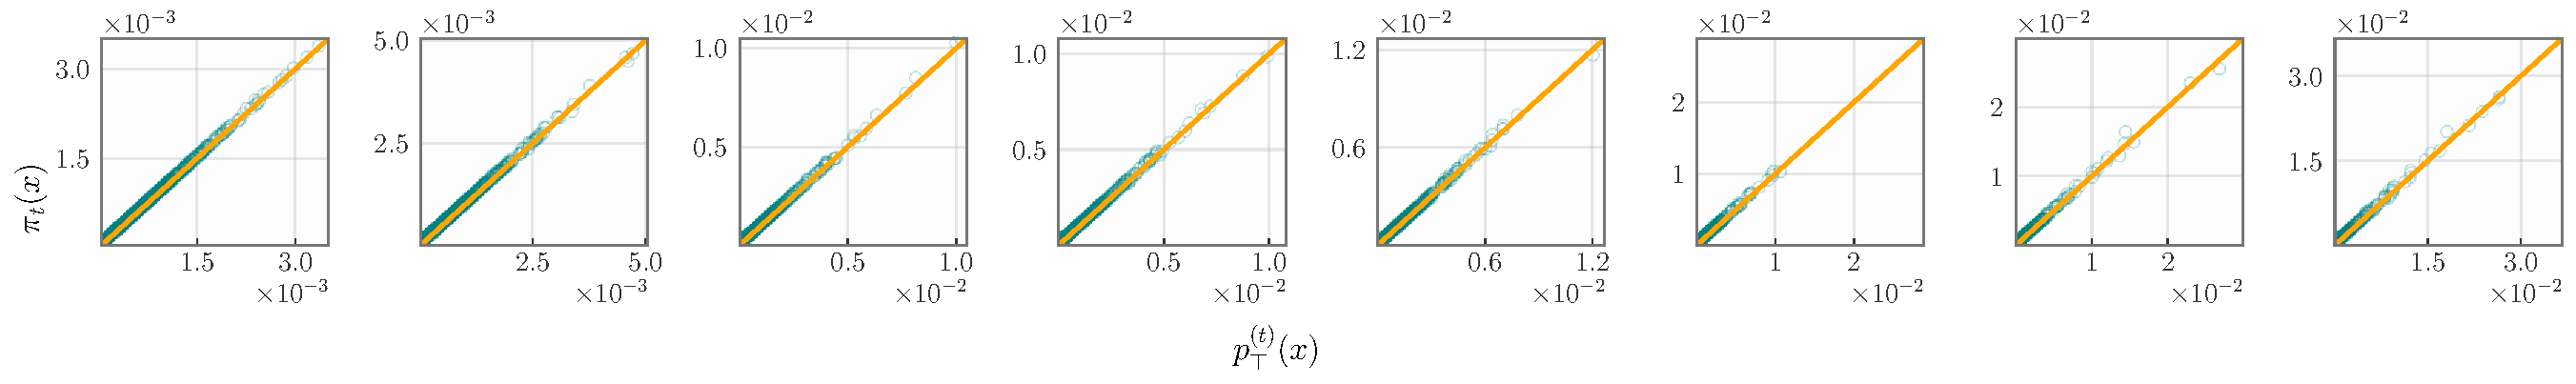
\includegraphics[width=\textwidth]{figures/streaming_eval_sets.py_plot.pdf}
    \caption{\textbf{SB-GFlowNets learn an accurate approximation to a changing target} distribution in a streaming setting for the task of set generation. Each plot depicts the target and learned distributions from the first (left-most) to the last (right-most) streaming update.}
    \label{fig:sets}
\end{figure}
\noindent\textbf{Problem description.} We first remark that, if $R_{1}, \dots, R_{k + 1}$ are positive functions on $\mathcal{X}$, the problem of streaming Bayesian inference may be generalized to the problem of sampling from $\mathcal{X}$ proportionally to the product $\prod_{i=1}^{k + 1} R_{i}$ by having only access to $R_{k + 1}$ and to a GFlowNet approximating $\prod_{i=1}^{k} R_{i}$. Indeed, in the context Bayesian inference, this correspondence is achieved by defining $R_{i}(x) \defeq f(\mathcal{D}_{i} | x)$ for $i > 1$ and $R_{1}(x) = f(\mathcal{D}_{1} | x) \pi(x)$.  
% We first remark that the problem of Bayesian inference under a streaming data setting may be equivalently framed as the problem of sampling proportionally to the product $\prod_{i=1}^{k + 1} R_{i}$ by having access only to a function $R_{k + 1}$ and to a GFlowNet trained to sample proportionally to $\prod_{i=1}^{k} R_{i}$ by letting $R_{i}(\cdot) = f(\mathcal{D}_{i} | \cdot)$ for $i > 1$ and $R_{1} (\cdot) = f(\mathcal{D}_{1} | \cdot) \pi(\cdot)$. 
Thus, to demonstrate the effectiveness of SB-GFlowNets and highlight the benefits and pitfalls of each proposed training scheme, we consider the set generation task --- a popular toy experiment in the GFlowNet literature \cite{Foundations, LingTrajectory, shen23gflownets}. In this task, $\mathcal{X}$ is the space of sets with $S$ elements extracted from a fixed deposit $\mathcal{I} = \{1, \dots, d\}$. Then, for $i \in \{1, \dots, K\}$, we define $f_{i} \colon \mathcal{I} \rightarrow \mathbb{R}$ and let $\log R_{i}(x) = \sum_{e \in x} f_{i}(e)$ be the $i$th log-reward of a set $x$. 

\pp{Experimental setup.} We fix $d = 24$ and $S = 18$. To define $R_{i}$, we independently sample $f_{i}(d)$ from an uniform distribution on $[-5, 5]$. Correspondingly, we define $R_{i}^{(\alpha)} \coloneqq R_{i}^{\nicefrac{1}{\alpha}}$ as the tempered reward, noting that $R_{i}^{(\alpha)}$ becomes increasingly sparse as $\alpha \rightarrow 0$. 

\captionsetup[table]{font=small}
\begin{wraptable}[6]{r}{.5\textwidth} 
    \centering
    \vspace{-12pt} 
    \caption{TV between the GFlowNet and the target. TB outperforms KL for sparse targets (small $\alpha$).} 
    \begin{tabular}{c|c|c|c}
         $\alpha$ &  $1.00$ & $0.75$ & $0.50$ \\
         \hline 
         TB & $0.21\textcolor{gray} { { \scriptstyle \pm 0.06 } }$& $0.28\textcolor{gray}{ {\scriptstyle \pm 0.10}}$ & $\mathbf{0.36}\textcolor{gray} {{\scriptstyle \pm  0.24}}$ \\ 
         KL & $\mathbf{0.13} \textcolor {gray} { { \scriptstyle \pm 0.03 } }$ & $\mathbf{0.17} \textcolor {gray} { { \scriptstyle \pm 0.04 } }$ & $0.55 \textcolor {gray} { { \scriptstyle \pm 0.38 } }$ 
    \end{tabular}
    \label{tab:sets}
\end{wraptable}
\captionsetup[table]{font=normal}
\pp{Results.} \autoref{tab:sets} highlights the differences between our two training schemes in terms of the target's temperature. For relatively sparse targets (with $\alpha < 1$), the benefits of off-policy sampling enacted by the minimization of the TB loss lead to a better performance relatively to the KL-minimizing algorithm. Indeed, the on-policy exploration employed by the latter potentially hinders the model's capabilities of finding the sparsely distributed high-probability regions of the target, slowing down the training convergence and potentially leading to mode collapse \cite{malkin2023gflownets}. Also, albeit one could implement an IS estimator for off-policy training under the KL criterion, our early experiments suggested that the increased gradient variance outweighed the gains from enhanced exploration. Ultimately, the choice of an appropriate learning objective for training GFlowNets will depend on the application. For training SB-GFlowNets, \autoref{fig:sets} shows that both TB and KL minimization result in accurate approximations to the changing posterior.  


% tb 0.5
% 0.72\textcolor { gray } { { \scriptstyle 0.48 } }
% tb 0.75
% 0.55\textcolor { gray } { { \scriptstyle 0.20 } }i
% tb 1.0
% 0.42\textcolor { gray } { { \scriptstyle 0.12 } }
% kl 0.5
% 1.10\textcolor { gray } { { \scriptstyle 0.76 } }
% kl 0.75
% 0.35\textcolor { gray } { { \scriptstyle 0.08 } }
% kl 1.0
% 0.26\textcolor { gray } { { \scriptstyle 0.07 } }

\subsection{Linear preference learning with integer-valued features} \label{sec:exp:p} 
\renewcommand{\pp}[1]{\noindent\textbf{#1}}

\pp{Problem description.} Consider a collection of instances $\{y_{i}\}$ endowed with a transitive and complete preference relation  $\succeq$; we assume that each $y_{i} \in \{1, 0\}^{d}$ is a binary feature vector. Naturally, the preference relation $\succeq$ is represented as a mapping $u$ such that $y \succ y^{\prime}$ if and only if $u(y) > u(y^{\prime})$; uncovering $u$ is the major goal of preference learning methods. Similarly to \cite{Cole1993, Hornberger1995}, we here assume that $u$ is a linear function, $u(y) = x^{T}y$, for a integer-valued vector $x$ and that we have access to a data set $\mathbf{y} = \{(y_{i1}, y_{i2}, p_{i})\}_{i}$ denoting whether $y_{i1}$ is preferred to $y_{i2}$ ($p_{i} = 1$) or otherwise ($p_{i} = 0$) for a fixed individual. Subsequently, we define the probabilistic model 
\begin{equation}
    p(p_{i} = 1 | x, (y_{i1}, y_{i2})) \coloneqq \sigma(u(y_{i1}) - u(y_{i2})) = \sigma\left(x^T (y_{i1} - y_{i2})\right), 
\end{equation}
in which $\sigma$ is the sigmoid function, and a prior distribution $\pi(x)$ over $x$ \cite{gonzalez2017preferential}; the intuition is that a larger difference between $y_{i1}$ and $y_{i2}$'s utilities makes the event in which $y_{i1}$ is preferred over $y_{i2}$ more likely. Our goal is to infer the individual's preferences based on the posterior $\pi(x | \mathbf{y})$ for some unseen pair $(\tilde{y}_{1}, \tilde{y}_{j})$, i.e., to estimate the predictive distribution $p(\tilde{y} | (\tilde{y}_{1}, \tilde{y}_{2}), \mathbf{y})$.  

\pp{Experimental setup.} We assume $x \in [[0, 4]]^{d}$ and $d = 24$. At each iteration of the streaming process, we sample a novel subset of the $2^{d - 1} \cdot (2^{d} - 1)$ pairs of $d$-dimensional binary feature vectors and use them to update the GFlowNet. The prior on $x$ is a factorized truncated Poisson with $\lambda = 3$. 

% Write about the generative process implemented by the GFlowNet. Also, describe the specific instantiations for the prior distributions. The architecture of the GFlowNet's policies, and the training details, should be described. The method for initializing the log-partition function, based upon their sequential structure, should be included somewhere around this properly edited document for experimental documentation. 
\begin{figure*}[!t] 
    \centering
    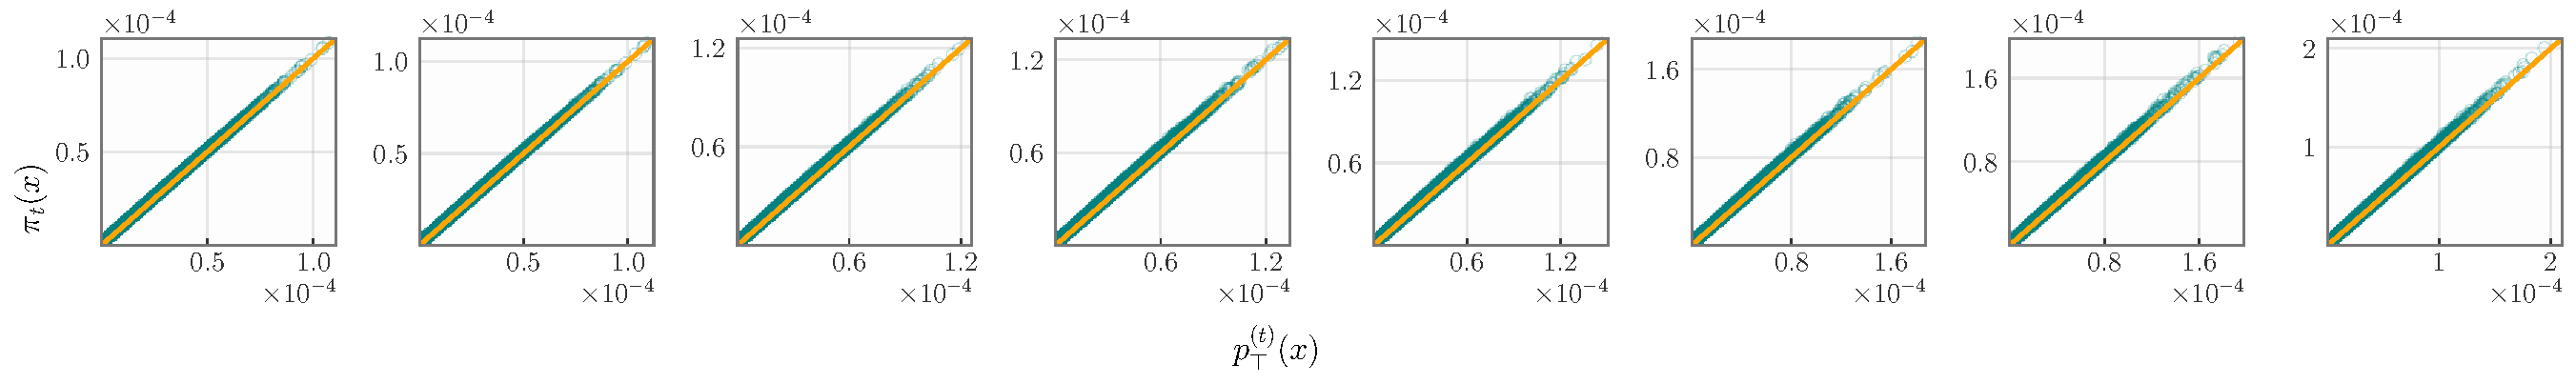
\includegraphics[width=\textwidth]{figures/distributional_approx.pdf}
    \caption{\textbf{SB-GFlowNet accurately learns the posterior over the utility's parameters in a streaming setting.} Each plot compares the marginal distribution learned by SB-GFlowNet (horizontal axis) and the targeted posterior distribution (vertical axis) at increasingly advanced stages of the streaming process, i.e., from $\pi_{1}( \cdot | \mathcal{D}_{1})$ (left-most) to $\pi_{8}(\cdot | \mathcal{D}_{1:8})$ (right-most).} 
    \label{fig:pref:dist}
\end{figure*}
\captionsetup[figure]{font=small}
\begin{wrapfigure}[11]{r}{.48\textwidth}  
    \centering
    \vspace{-8pt} 
    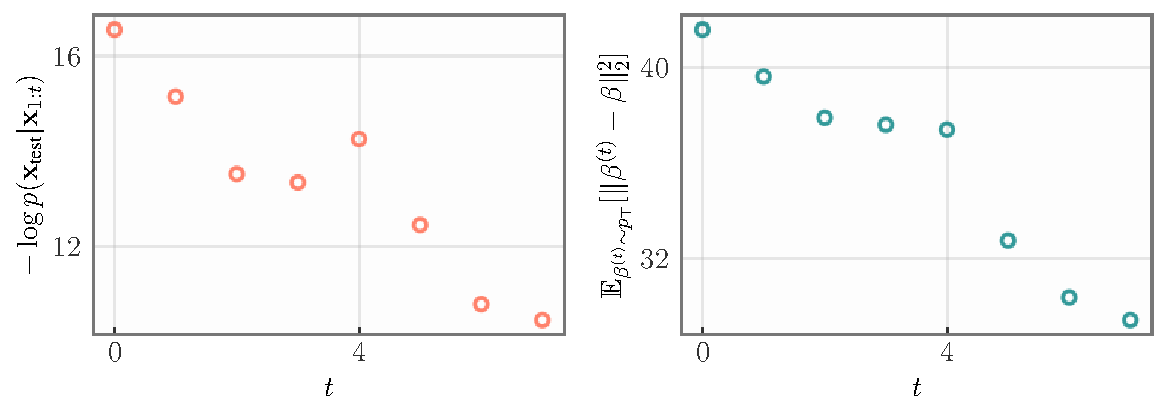
\includegraphics[width=\linewidth]{figures/predictive_nll_preferences.pdf} 
        \caption{Predictive performance of SB-GFlowNets in terms of pred. NLL and avg. MSE. SB-GFlowNets behaves similarly to the ground-truth, wrt how the NLL evolves as a function of data chunks.} % {Both the predictive NLL on a test data set (\textcolor{brickred}{left}) and the avg. MSE between the predicted and true parameter of the utility (\textcolor{teal}{right}) decrease as a function of streaming updates.}
    \label{fig:pref:p}
    \vspace{-15pt} 
\end{wrapfigure}
\captionsetup[figure]{font=normal}
\pp{Results.} \autoref{fig:pref:dist} shows SB-GFlowNet correctly % learns 
samples form the posterior % distribution 
in a streaming setting. Note, in particular, that the GFlowNet maintains a high distributional accuracy throughout the streaming iterations. Correspondingly, the predictive log-likelihood of a fixed held out data set monotonically increases as a function of the amount of data consumed by the SB-GFlowNet, as shown in \autoref{fig:pref:p}; this behavior, also exhibited by the true posterior \cite{Walker1969}, emphasizes the similarity between the learned and targeted distributions. \looseness=-1 

% Possibly include something about an inadequate training at an early stage leading to inadequate training at later stages 

\subsection{Online Bayesian phylogenetic inference} \label{sec:exp:i} 
\renewcommand{\pp}[1]{\vspace{0pt}\noindent\textbf{#1}}

\pp{Problem description.} Bayesian phylogenetic inference (BPI) \cite{zhang2018variational, kviman2024improved} aims to infer structural properties of evolutionary trees given molecular sequences such as DNA and RNA. Formally, let $\{S_{1}, \dots, S_{N}\}$ be a collection of $N$ DNA sequences of size $M$, $S_{i} \in \{A, T, C, G\}^{M}$, one for each biological species. We define a \textit{phylogeny} as a tuple $T = (t, \mathbf{b})$ comprising a \textit{rooted tree topology} $t$ and its non-negative \textit{branch lengths} $\mathbf{b}$. In this context, a rooted tree topology is a complete binary tree having $N$ labeled leaves corresponding to the considered species and $N - 1$ unlabeled internal nodes corresponding to their ancestors. To carry out Bayesian inference over the space of phylogenies, we adopt Jukes \& Cantor's nucleotide substitution model (JC69; \cite{Jukes1969}) to define a observational model over the observed DNA sequences; to calculate the likelihood, we use Felsenstein's algorithm~\cite{Felsenstein1981}. \looseness=-1 

% To marginalize out the unobserved data, we implement Felsenstein's algorithm [ref].  
% Explicitly, a phylogeny is this, this and that 
% The Bayesian likelihood model is typically based on a substitution model (we use JC69) 
% The likelihood is computed through the dynamically programmed Felsenstein's algorithm
% The space of trees is combinatorial and sampling from this posterior is often an unachievable goal 

Crucially, despite the popularity of BPI methods, the development of new sequencing technologies has swiftly led to the enlargement of already sizeable sequence databases. In this scenario, maintaining an up-to-date estimate of the posterior became an increasingly difficult task due to the necessity of re-estimating the full posterior from scratch every time a new batch of data is collected. In the following, we show that GFlowNets, which have recently shown SOTA performance in BPI \cite{zhou2024phylogfn}, can also accurately update the posterior on phylogenetic trees given additional sequences. 

\pp{Experimental setup.} We generate the data by simulating JC69's model for a collection of $N = 7$ species and a substitution rate of $\lambda = 5 \cdot 10^{-1}$ (see \cite{Yang2014}, Chapter 1). At each iteration, we sample a new DNA subsequence of size $10^{2}$ for each species and update SB-GFlowNet according to \autoref{alg:training}. For \autoref{tab:phy:t}, $|\mathcal{D}_{1}| = 10^{3}$ and $|\mathcal{D}_{2}| = 10^{2}$. The prior is an uniform distibution over phylogenies. % The models were trained for $20000$ epochs with a batch size of $128$ to estimate the stochastic gradients. 

% Write about the generation of the data, the discretization of the branch lengths, the number of leaves, the number of sites, the hyperparameters of Junkes' models 

% \begin{wrapfigure}[7]{r}{.5\textwidth} 
%     \centering
%     \vspace{-12pt} 
%     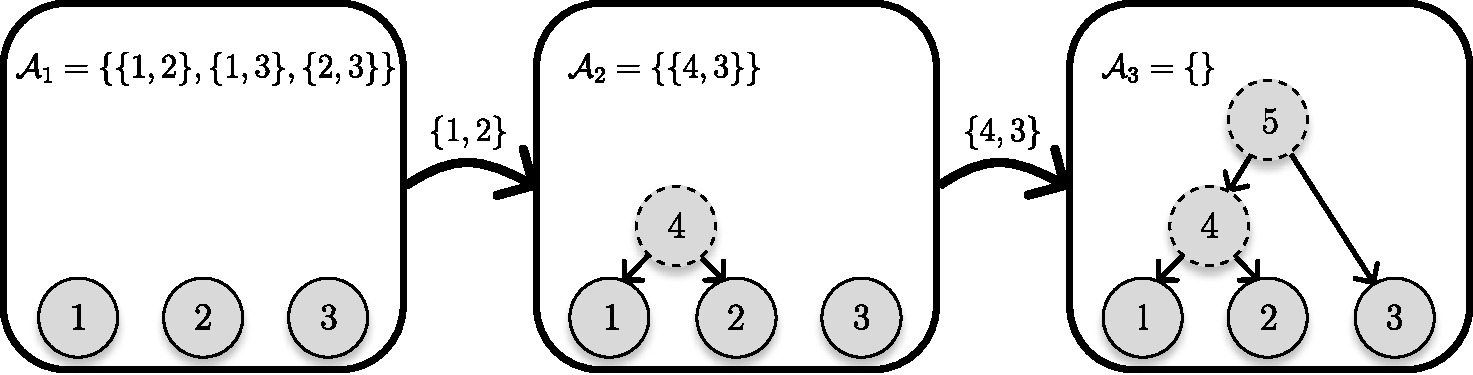
\includegraphics[width=\linewidth]{figures/phylogenies.pdf}
%     \caption{Generative process for phylogenies.} % The initial state is a forest of singleton trees represented by the leaves (left). To generate a topology, we iteratively join the roots of two trees (middle) until the graph becomes weakly connected (right).}
%     \label{fig:phy:trees}
%     \vspace{-12pt} 
% \end{wrapfigure}

% For generative  A state consists of a forest of binary complete trees. 

\captionsetup[figure]{font=small}
\begin{wrapfigure}{r}{.5\textwidth} 
    \centering
    \vspace{-12pt} 
    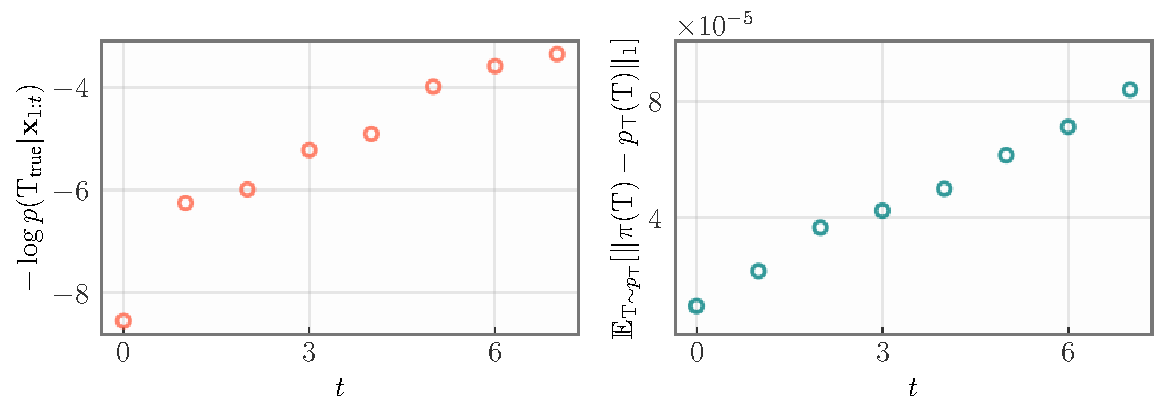
\includegraphics[width=\linewidth]{figures/phylogenetics_dist_approx.pdf}
    \caption{SB-GFlowNet's accurate fit to the true posterior in terms of the probability of the true phylogeny (left) and of the learned model's accuracy (right).}
    \label{fig:phy:dist}
    \vspace{-10pt} 
\end{wrapfigure}
\captionsetup[figure]{font=normal}
\pp{Results.} \autoref{fig:phy:dist} (left) shows that the learned posterior distribution gets increasingly concentrated on the true phylogenetic tree; this behavior, which is inherent to posteriors over phylogenies under uniform priors \cite{roychoudhury2015}, emphasizes the similarity between the learned and targeted distributions for SB-GFlowNets. \autoref{fig:phy:dist} (right), on the other hand, also suggets that the model's accuracy decreases as a function of the number of streaming updates. Nonetheless, we believe that this is predominantly caused by the posterior's increasing sparsity due to the expanding data sets \cite{roychoudhury2015}, which makes it more difficult for the GFlowNet to learn a good approximation \cite{deleu2022bayesian}, instead of by an intrinsic limitation of SB-GFlowNets. % Indeed, we noted that SB-GFlowNet leads to a \textit{better} approximation to the posterior than a standard GFlowNet trained to sample from the full posterior under the same computational budget. 
An investigation of this phenomenon and of the conditions upon which re-train the SB-GFlowNet based on an earlier checkpoint due to the accumulated unreliability of the streaming updates, as described by \autoref{prop:aaa}, is left application-dependent and is thereby left to future endeavors. 
% 
Finally, \autoref{tab:phy:t} shows that SB-GFlowNets, which avoids evaluating the full posterior, more than halve the training time required by a standard GFlowNet, while achieving a similar performance in terms of the total variation ($TV$) distance between the learned and target distributions.  

% This, together with \cite{zhou2024phylogfn}, identifies GFlowNets as a general and scalable framework for BPI that may potentially be a better alternative than MCMC methods such as the ones proposed by \cite{Dinh2017, Bouckaert2019}. Importantly, in contrast with MCMC-based approaches, GFlowNets are natively compatible with GPU-based high-performance computing. %  and provide a computationally efficient and unbiased estimator for a sample's density (see Equation [ref]).   

\begin{table}[t!] 
    \centering
    \caption{\textbf{SB-GFlowNet significantly accelerates the training of GFlowNets} in a streaming setting. Indeed, SB-GFlowNets achieve an accuracy comparable to a GFlowNet trained from scratch to sample from $\pi_{2}(\cdot | \mathcal{D}_{1:2})$ in less than half the time (measured in seconds per $20$k epochs).}  
    \begin{tabular}{lccc}
        & \multicolumn{3}{c}{Number of leaves} \\ \cmidrule(lr){2-4} 
        Model & 7 & 9 & 11 \\ \midrule  
        GFlowNet &  $2846.88$ {\small\color{gray}\emph{s}} & $3779.11$ {\small\color{gray}\emph{s}}& $4821.74$ {\small\color{gray}\emph{s}}\\ 
        SB-GFlowNet (\textit{ours}) & $\mathbf{1279.68}$ {\small\color{gray}\emph{s}}& $\mathbf{1714.49}$ {\small\color{gray}\emph{s}}& $\mathbf{2303.99}$ {\small\color{gray}\emph{s}}\\  
        \midrule
        Relative accuracy gain (TV) & $0.00 \textcolor{gray}{ { \scriptstyle \pm 0.04 } }$ & $-0.02 \textcolor{gray}{ { \scriptstyle \pm 0.04 } }$ & $0.00 \textcolor{gray}{ { \scriptstyle \pm 0.01 } }$ 
    \end{tabular}
    % {The time (in seconds per $20000$ epochs) to train a standard model to sample from $\pi_{2}(\cdot | \mathcal{D}_{1:2})$ is more than twice as high as SB-GFlowNet's training time.}
    \label{tab:phy:t}
    % \vspace{-12pt} 
\end{table}

\subsection{Bayesian structure learning} \label{sec:exp:c}

\begin{figure}[h!]
    \centering
    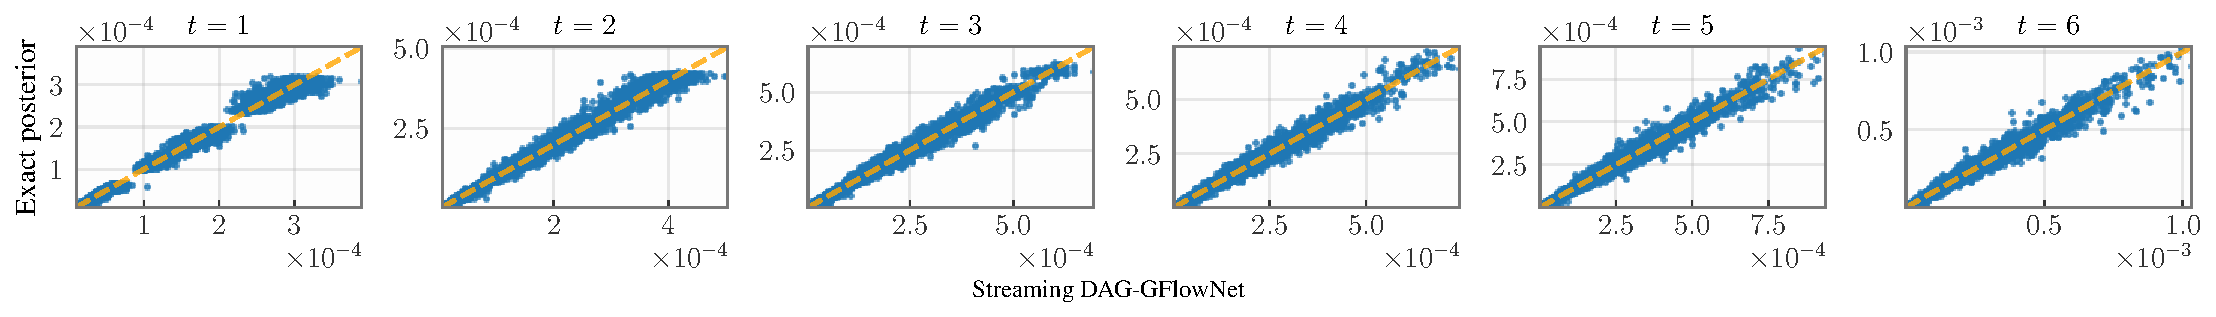
\includegraphics[width=.9\linewidth]{figures_rebuttal/streaming_eval_dags.pdf}
    \caption{\textbf{SB-GFlowNets accurately learns a distribution over DAGs} 
    for causal discovery in each time step. At each update, an additional dataset of $200$ points was sampled from the true model. For this problem, we implemented a DAG-GFlowNet on $5$-variable data sets, similarly to \cite[Figure 3]{deleu2022bayesian}. \looseness=-1}
    \label{fig:dagscausal}
\end{figure}

\pp{Problem description.} Let $\mathbf{X} \in \mathbb{R}^{n \times d}$ be a data set distributed according to a linear Gaussian structural equation model (SEM), i.e., $\mathbf{X} = \beta \mathbf{X} + \boldsymbol{\epsilon}$, in which $\beta \in \mathbb{R}^{d \times d}$ is a (sparse) matrix and $\boldsymbol{\epsilon} \in \mathbb{R}^{n \times d}$ are $nd$ i.i.d. samples from a normal distribution. We assume that the adjacency matrix induced by $\beta$, $[\beta \neq 0] \in \{1, 0\}^{d \times d}$, characterizes a directed acyclic graph on the dataset's variables. In this case, the linear Gaussian SEM represents a Bayesian network, and it is the goal of \emph{Bayesian structure learning} algorithms to find such a network based on the observed $\mathbf{X}$ \cite{deleu2022bayesian}. Although this problem has been studied beyond the constraints of linear models governed by Gaussian distributions \cite{deleu2023joint}, we focus on a simplified setting in this section. In particular, given a sequence $\{\mathbf{X}_{t}\}_{t \ge 1}$ of i.i.d. realizations of a linear Gaussian SEM, we define a belief distribution over Bayesian networks $\mathcal{N} = (\{1, \dots, d\}, \mathbf{A})$ on variables $\{1, \dots, d\}$ and adjacency matrix $\mathbf{A}$ as \looseness=-1 
\begin{equation}
    \log R_{t}(\mathcal{N}) = \max_{\beta \colon [\beta \neq 0] = \mathbf{A}} \ell \left( \beta | \mathbf{X}_{t} \right) \text{ and } R_{1:t}(\mathcal{N}) = \prod_{1 \le i \le t} R_{t}(\mathcal{N}), % .     
\end{equation}
in which $\ell(\beta | \mathbf{X}_{t})$ is the log-likelihood of $\mathbf{X}_{t}$ under the linear Gaussian SEM parameterized by $\beta$. 
SB-GFlowNets can naturally handle streaming inference for this model by casting each $R_{t}$ as a subposterior distribution --- in the same fashion of the set generation task in \autoref{subsec:sets}.  
\looseness=-1 

% \looseness=-1         

\captionsetup[figure]{font=small}
\begin{wrapfigure}[13]{r}{.25\textwidth} 
    \vspace{-9pt} 
    \centering
    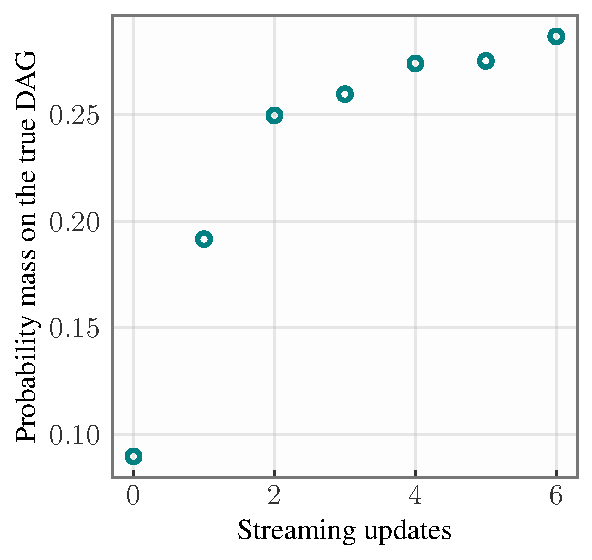
\includegraphics[width=\linewidth]{figures_rebuttal/streaming_eval_dags_true_dag_probability.pdf}
    \caption{The probability mass on the true DAG increases as more samples are added to SB-GFlowNet.}%  Results are based on the same experimental setup of Figure~\ref{fig:dagscausal}.} 
    \label{fig:tdagprob}
\end{wrapfigure}
\captionsetup[figure]{font=normal}
\pp{Experimental setup.} Likewise \citet[Figure 5]{deleu2022bayesian}, we evaluate SB-GFlowNets on models with $d = 5$ variables. Also, we sample a new $200$-sized data set from a fixed linear Gaussian SEM for each streaming update of the GFlowNet. To ensure that the generated samples are valid DAGs, we adopt \citet{deleu2022bayesian}'s DAG-GFlowNet. \looseness=-1 %  as the backbone of our SB-GFlowNet. 
% \looseness=-1    

\pp{Results.} Our results corroborate the findings of \autoref{sec:exp:i}. On the one hand, \autoref{fig:dagscausal} highlights that our SB-GFlowNet can accurately learn a distribution over DAGs across a range of streaming updates. %  and 
On the other hand, \autoref{fig:dagscausal} shows that the probability mass assigned by the SB-GFlowNet to the true DAG responsible for the data-generating process increases as more samples are incorporated into the belief distribution. Hence, SB-GFlowNets abide by the desiradata of a streaming algorithm for Bayesian inference. 
\looseness=-1  

\section{Related works} \label{sec:aa} 
\renewcommand{\pp}[1]{\noindent\textbf{#1}}

\pp{Applications of GFlowNets.} GFlowNets \cite{Foundations, Bengio2021, theory} were originally proposed as reinforcement learning algorithms to train a stochastic policy to sample states proportionally to a prescribed reward function, % contrasting with the customary reward-maximizing methods employed at the time. 
From this point on, GFlowNets were widely applied to problems as diverse as probabilistic modeling \cite{ discretegfn_ii, discretegfn_iii}, combinatorial optimization \cite{Zhang2023}, Bayesian causal discovery \cite{deleu2022bayesian, deleu2023joint} and phylogenetic inference \cite{zhou2024phylogfn}, symbolic regression \cite{li2023gfnsr}, stochastic control \cite{theory}, language modeling \cite{hu2023amortizing}, and Bayesian deep learning \cite{liu2023dropout}. 
Recently, there is an increasing literature concerned with the possibility of composing multiple pre-trained GFlowNets to fit them to specific applications \cite{garipov2023compositional} and to accelerate training convergence \cite{lau2023dgfn}. In this context, we show how the composition of two GFlowNets through the SB condition leads to an efficient learning algorithm for Bayesian inference under a streaming setting. \looseness=-1 

% Practice, practice and practice 

% train GFlowNets in a streaming setting by utilizing pre-trained GFlowNet on past data.   

\pp{Streaming Variational Bayes.} Streaming, Distributed, Asynchronous (SDA) Bayes \cite{Broderick13} was originally presented as a general framework for implementing variational inference algorithms in a streaming setting. Similarly to our work, it was based upon the principle that, if the variational distribution $q^{(t)}(x)$ is a good approximation to the unnormalized posterior $\tilde{\pi}_{t}(x)$, then $q^{(t + 1)}(x)$ may be optimized to approximate $q^{(t)}(x) f(\mathcal{D}_{t} | x)$ instead of $f(\mathcal{D}_{t} | x) \tilde{\pi}_{t}(x)$. This framework was instantiated to accommodate, for example, the learning of Gaussian processes \cite{bui2017GPs}, of tensor factorization \cite{Fang21Tensor}, of feature models \cite{Schaeffer22features} and, jointly with SMC, nonlinear state-space models \cite{Zhao2023}. Nonetheless, our work is the first one to enable the training of GFlowNets in a streaming setting and, due to the relationship between GFlowNets and variational inference algorithms presented by \cite{malkin2023gflownets}, may be viewed as an instance of SDA-Bayes tailored to inferential problems on a combinatorial support. 
In the realm of approximate Bayesian inference, \citet{sendera2024diffusion, berner2022optimal, akhound2024iterated, zhang2018variational} propose advancements in diffusion-based sampling methods, which we believe could be extended to the context of approximate streaming Bayesian inference via the techniques presented in this work. 
On the other hand, \citet{mittal2023exploring} introduces an neural network-based approach for approximate Bayesian inference that amortizes over exchangeable data sets to handle posterior inference in novel data.  
Also, \citet{richter2023improved, richter2020vargrad} develop a low-variance gradient estimator for carrying out variational inference derived from the \emph{log-variance loss}, which could be employed as an alternative to our KL-based objective for streaming updates of GFlowNets. 
On a broader scale, \citet{cranmer2020frontier} reviews approximate Bayesian methodology under the lens of simulation-based inference.  
\looseness=-1 
% In the realm of approximate Bayesian inference, we refer the reader to \cite{cranmer2020frontier, mittal2023exploring, zhang2018variational, richter2020vargrad, sendera2024diffusion, berner2022optimal, akhound2024iterated, richter2023improved}. 

% \begin{proposition}[SB-GFlowNets and SDA-Bayes] \label{prop:sda} 
%     There exist a variational family of distributions and a learning algorithm for which SDA-Bayes becomes a SB-GFlowNet. 
% \end{proposition}

\section{Conclusions, limitations, and outlook} \label{sec:aaa} 



\pp{Conclusions.} We proposed the first method for carrying out approximate Bayesian inference over discrete distributions within a streaming setting, called SB-GFlowNet. We proposed two training/update schemes for SB-GFlowNet, as well as a theoretical analysis accounting for the compounding effect of errors due to posterior propagation. 
%
Our experimental evaluation showcases SB-GFlowNet`s effectiveness in accurately sampling from the target posterior --- while still achieving a significant reduction in training time relative to standard GFlowNets.
%

\pp{Limitations.} \autoref{prop:a} and \autoref{prop:aaa} suggest that an inappropriate approximation to $\pi_{t}$ may be propagated through time and lead to increasingly inaccurate models. This phenomenon, known as \emph{catasthropic forgetting} in the online literature \cite{McCloskey1989,Goodfellow2014}, may eventually demand retraining of the current SB-GFlowNet based on an earlier checkpoint or on the full posterior.
%
We also note that unlike traditional variational methods, where the expressiveness of the approximation family is explicitly chosen, the expressiveness implied by different parametrizations of GFlowNets is not clear. We believe this is a fruitful avenue for future investigation.

% However, all of our results and algorithms remain valid if we substitute $p_{\top}^{(t)}$ (resp. $p_{F}^{(t)}$) by $p_{\top}^{s}$ (resp. $p_{F}^{s}$) and $\mathcal{D}_{t + 1}$ by $\bigcup_{i=s + 1}^{t + 1}\mathcal{D}_{i}$ for any checkpoint $s < t$. 

\pp{Outlook and future works}
As our proposal provides generic and efficient streaming variational inference solution for discrete parameters, we believe it will allow the use of streaming discrete Bayesian inference to more datasets and to less explored research domains.
% 
In this work, we proposed two training criteria based on the trajectory balance condition and the KL criterion, nonetheless, these are not the only training schemes for GFlowNets, we believe other proposed criteria such as \emph{detailed balance}~\citep{Foundations} or the \emph{sub-trajectory balance}~\cite{Madan2022LearningGF} could be adapted for the streaming setting as well.
%
Additionally, due to the flexibility of GFlowNets in sampling unnormalized distributions, our proposal can be extended to different divergences and generalized likelihoods to improve the predictive quality of the learned posteriors \cite{Knoblauch2022}. Finally, the problem of updating a GFlowNet when the size of the generated object changes, e.g., when a new species is observed during BPI, remains open. \looseness=-1   


\section*{Acknowledgements}

This work was supported by the Fundação Carlos Chagas Filho de Amparo à Pesquisa do Estado do Rio de Janeiro FAPERJ (SEI-260003/000709/2023), the São Paulo Research Foundation FAPESP (2023/00815-6), the Conselho Nacional de Desenvolvimento Científico e Tecnológico CNPq (404336/2023-0), and the Silicon Valley Community Foundation through the University Blockchain Research Initiative (Grant \#2022-199610).

% \clearpage

\bibliographystyle{abbrvnat} 
\bibliography{bibliography} 

\newpage 
\onecolumn 

\appendix

% \subsection{Uniform distributions and uniform flows}
\begin{itemize}
    \item A uniform flow of degree $g$ and height $h$ is a Markovian flow that models a uniform distribution, meaning all the leaf nodes have the same value. The policy of such flow consists in a function that takes the incoming flow and splits it equally between each of the g outgoing nodes.
\end{itemize}

To start let us consider the example of a flow trained on a uniform distribution and policy that takes the incoming flow and split it equally to all outgoing states. The resulting uniform distribution on the terminal nodes density is  represented by $\pi^*(x)=\frac{1}{g^h}$, for each terminal object in the domain $x \in \mathcal{X}$ and $|\mathcal{X}|=g^h$.

Let us consider the case that the policy at the root of the network introduces an error in the flow of size $\delta$, meaning that one children node now will receive a flow $\frac{F}{g}+\delta$ and the other $g-1$ will continue with $\frac{F}{g}$, which is equivalent to the policy with a probability density (after normalizing) that assigns a probability $\frac{F+g\delta}{g(F+\delta)}$ to one branch and $\frac{F}{g(F+\delta)}$ to the other $g-1$ branches. The total variation distance between this new density and the original policy (uniform probability for each $g$ branches) is $\epsilon(\delta, g)=(1-\frac{1}{g})\frac{\delta}{F+\delta}$. Now we denote the resulting sampling distribution induced by this modified flow as $\pi(x)$.


\begin{figure}[h]
    \center 
% https://q.uiver.app/#q=WzAsMTMsWzMsMCwiRitcXGRlbHRhIl0sWzIsMSwiXFxmcmFje0Z9e2d9K1xcZGVsdGEiXSxbNCwxLCJcXGZyYWN7Rn17Z31cXHRleHR7IH1cXHRyaWFuZ2xlIl0sWzIsMiwiXFx0cmlhbmdsZSJdLFswLDMsIlxcZnJhY3tGfXtnXmh9K1xcZGVsdGFfMSJdLFsxLDIsIlxcdHJpYW5nbGUiXSxbNSwyLCJcXHRyaWFuZ2xlIl0sWzQsMiwiXFx0cmlhbmdsZSJdLFsxLDMsIlxcZnJhY3tGfXtnXmh9K1xcZGVsdGFfMlxcdGV4dHsgIH1cXGxkb3RzICJdLFsyLDMsIlxcZnJhY3tGfXtnXmh9K1xcZGVsdGFfe2dee2gtMX19Il0sWzQsMywiXFxmcmFje0Z9e2deaH0iXSxbNSwzLCJcXGZyYWN7Rn17Z15ofSJdLFs2LDMsIlxcZnJhY3tGfXtnXmh9Il0sWzAsMSwiXFx0ZXh0e2RlZ3JlZSBnfSJdLFswLDJdLFsyLDZdLFsyLDddLFsxLDNdLFsxLDVdLFs1LDRdLFs1LDhdLFszLDldLFs3LDEwXSxbNiwxMV0sWzYsMTJdXQ==
\[\begin{tikzcd}
	&&& {F+\delta} \\
	&& {\frac{F}{g}+\delta} && {\frac{F}{g}\text{ }\triangle} \\
	& \triangle & \triangle && \triangle & \triangle \\
	{\frac{F}{g^h}+\delta_1} & {\frac{F}{g^h}+\delta_2\text{  }\ldots } & {\frac{F}{g^h}+\delta_{g^{h-1}}} && {\frac{F}{g^h}} & {\frac{F}{g^h}} & {\frac{F}{g^h}}
	\arrow["{\text{degree g}}", from=1-4, to=2-3]
	\arrow[from=1-4, to=2-5]
	\arrow[from=2-5, to=3-6]
	\arrow[from=2-5, to=3-5]
	\arrow[from=2-3, to=3-3]
	\arrow[from=2-3, to=3-2]
	\arrow[from=3-2, to=4-1]
	\arrow[from=3-2, to=4-2]
	\arrow[from=3-3, to=4-3]
	\arrow[from=3-5, to=4-5]
	\arrow[from=3-6, to=4-6]
	\arrow[from=3-6, to=4-7]
\end{tikzcd}\]
\caption{A flow network with a extra flow of $\delta$ in one of the branches of the initial state} 
    \label{fig:tree_graph} 
\end{figure}

Let $\mu$ and $\nu$ be two probability measures, then we denote $||\mu - \nu||_{\scaleto{\textbf{TV}}{3pt}}$ as the total variation distance between them. 

\begin{assumption}\label{as: gf_tree_unif}
 Let the pair $(G_T, F)$ be a flow network such that $G_T$ is a regular tree with degree $g$ and depth $h$. Furthermore, assume that $F$ spreads uniformly in the edges of $G_T$, then the target distribution $\pi^*$ generated by $(G_T, F)$ is uniform.      
\end{assumption}

\begin{theorem}[Total variation of the sampling distribution] Let $\delta >0$ and $\sum_{i=1}^{g^{h-1}} \delta_i = \delta$, where $\delta_i \in [0, \delta]$ for all $i \in \{1,2, \dots, g^{h-1}\}$. Suppose that we have the flow network $(G_T, F+\delta)$  abiding by Assumption~\ref{as: gf_tree_unif} besides the first edge from the root to a son where it has a $\delta$ increasing generating a new target distribution $\pi$. Then under these conditions describe the total variation distance between $\pi$ and $\pi^*$ is bounded above and below by the following
\begin{align*}
& \epsilon(\delta, g) \leq ||\pi - \pi^*||_{\scaleto{\textbf{TV}}{3pt}} \leq \epsilon(\delta, g^h) \quad \text{where}
\\
& \epsilon(a,b) := \Big(1 - \frac{1}{b} \Big) \frac{a}{F+a}\,.
\end{align*}
\end{theorem}

\begin{proof}
The terminal states of the modified flow network will have two types of nodes, with flow $\frac{F}{g^h}$ and $\frac{F}{g^h}+\delta_{i}$, with $\delta_i \geq 0$ and $\sum_{i=1}^{g^{h-1}} \delta_i = \delta$. We normalize those probabilities to obtain the individual probabilities for each terminal state, which determines the density of each sample. From that, we can proceed to compute the total variation distance between $\pi$ and $\pi^*$.
\begin{align*}
    ||\pi - \pi^*||_{\scaleto{\textbf{TV}}{3pt}} &= \frac{1}{2}\sum_{x \in \mathcal{X}} | \pi(x)- \pi^*(x) | \\
                          &= \frac{1}{2}\left[(g^h-g^{h-1})\left|\frac{F}{g^h}\frac{1}{F+\delta} - \frac{1}{g^h}\right|+ \sum_{i=1}^{g^{h-1}} \left|\frac{F+g^h\delta_i}{g^h}\frac{1}{F+\delta} - \frac{1}{g^h}\right| \right] \\
                          &= \frac{1}{2}\left[\frac{g^h\delta-g^{h-1}\delta+\sum_{i=1}^{g^{h-1}}|g^h\delta_i-\delta|}{g^h(F+\delta)}\right]
\end{align*}

We can lower bound $\sum_{i=1}^{g^{h-1}}|g^h\delta_i-\delta|$, by considering that $\sum_{i=1}^{g^{h-1}}(g^h\delta_i-\delta)=g^{h}\delta-g^{h-1}\delta$, taking the absolute value of the result and each element of the sum to obtain $g^{h}\delta-g^{h-1}\delta \leq \sum_{i=1}^{g^{h-1}}|g^h\delta_i-\delta|$. Thus we obtain the lower bound 
\begin{align*}
\frac{1}{2}\left[\frac{g^h\delta-g^{h-1}\delta+g^{h}\delta-g^{h-1}\delta}{g^h(F+\delta)}\right]&\leq \frac{1}{2}\left[\frac{g^h\delta-g^{h-1}\delta+\sum_{i=1}^{g^{h-1}}|g^h\delta_i-\delta|}{g^h(F+\delta)}\right] \\
                       \left(1-\frac{1}{g}\right)\frac{\delta}{F+\delta} &\leq  ||\pi - \pi^*||_{\scaleto{\textbf{TV}}{3pt}} 
\end{align*}.

This lower bound is reached when all error terms in the terminal states have the same value $\delta_i = \frac{\delta}{g^h}$.

To upper bound $|g^h\delta_i-\delta|$ we apply the triangle inequality, obtaining $|g^h\delta_i-\delta| \leq g^h\delta_i+\delta$ and  $\sum_{i=1}^{g^{h-1}}|g^h\delta_i-\delta| \leq g^h\delta+g^{h-1}\delta$, from which we obtain the upper bound
\begin{align*}
    ||\pi - \pi^*||_{\scaleto{\textbf{TV}}{3pt}} &\leq \frac{1}{2}\left[\frac{g^h\delta-g^{h-1}\delta + g^{h}\delta+g^{h-1}\delta}{g^h(F+\delta)}\right] \\
    ||\pi - \pi^*||_{\scaleto{\textbf{TV}}{3pt}} &\leq \frac{\delta}{F+\delta}
\end{align*}.

To obtain a tighter bound we break the sum $\sum_{i=1}^{g^{h-1}}|g^h\delta_i-\delta|$ by partitioning the sum into the first $I$ terms $S_A=g^h\sum_{i=1}^{I}|\delta_i-\frac{\delta}{g^h}|$ with $\delta_i < \frac{\delta}{g^h}$ and subsequent $g^{h-1}-I$ terms $S_B=g^h\sum_{j=I+1}^{g^{h-1}}|\delta_j-\frac{\delta}{g^h}|$ with $\delta_j \geq \frac{\delta}{g^h}$. By construction, we know that $S_A+g^h\sum_{i=1}^{I}\delta_i+g^h\sum_{j=I+1}^{g^{h-1}}\delta_j-S_B=g^{h-1}\delta$, simplifying to $S_B-S_A=\delta(g^h-g^{h-1})$. We rewrite $S_A + S_B = S_B-S_A+2S_A=\delta(g^h-g^{h-1})+2S_A$, and by triangle inequality on $S_A$, we obtain the upper bound $\sum_{i=1}^{g^{h-1}}|g^h\delta_i-\delta|=S_A+S_B \leq g^h\delta-g^{h-1}\delta+2I\delta $. Setting $I=g^{h-1}-1$ (the biggest value it can have without breaking the constraints on $\delta_i$), it simplifies to $S_A+S_B \leq g^h\delta+g^{h-1}\delta-2\delta $

\begin{align*}
    ||\pi - \pi^*||_{\scaleto{\textbf{TV}}{3pt}} &\leq \frac{1}{2}\left[\frac{g^h\delta-g^{h-1}\delta+\sum_{i=1}^{g^{h-1}}|g^h\delta_i-\delta|}{g^h(F+\delta)}\right] \\
    ||\pi - \pi^*||_{\scaleto{\textbf{TV}}{3pt}} &\leq \frac{1}{2}\left[\frac{g^h\delta-g^{h-1}\delta+g^h\delta+g^{h-1}\delta-2\delta }{g^h(F+\delta)}\right] \\
    ||\pi - \pi^*||_{\scaleto{\textbf{TV}}{3pt}} &\leq \left[\frac{g^h\delta-\delta }{g^h(F+\delta)}\right] \\
    ||\pi - \pi^*||_{\scaleto{\textbf{TV}}{3pt}} &\leq  \left(1-\frac{1}{g^h}\right)\frac{\delta}{F+\delta}
\end{align*}.
\end{proof}

\textcolor{red}{\begin{theorem}[Total variation of the sampling distribution] Let $\delta >0$ and $\sum_{i=1}^{n} \delta_i = \delta$, where $\delta_i \in [0, \delta]$. Suppose that we have the flow network $(G_n, F)$ which generates a target distribution $\pi^*$ uniform in the number of final vertices. Then if we increase the flow $F$ by $\delta$ in the same graph, that is $(G_n, F + \delta)$, generating a new target distribution $\pi$, the total variation distance between $\pi$ and $\pi^*$ is bounded above and below by the following
\begin{align*}
& ||\pi -\pi^*||_{\scaleto{\textbf{TV}}{3pt}} \leq \epsilon(\delta, n) \quad \text{where}
\\
& \epsilon(a,b) := \Big(1 - \frac{1}{b} \Big) \frac{a}{F+a}\,.
\end{align*}
\end{theorem}}




\section{Inherent limitations of policy networks}



\begin{figure}
    \center 
    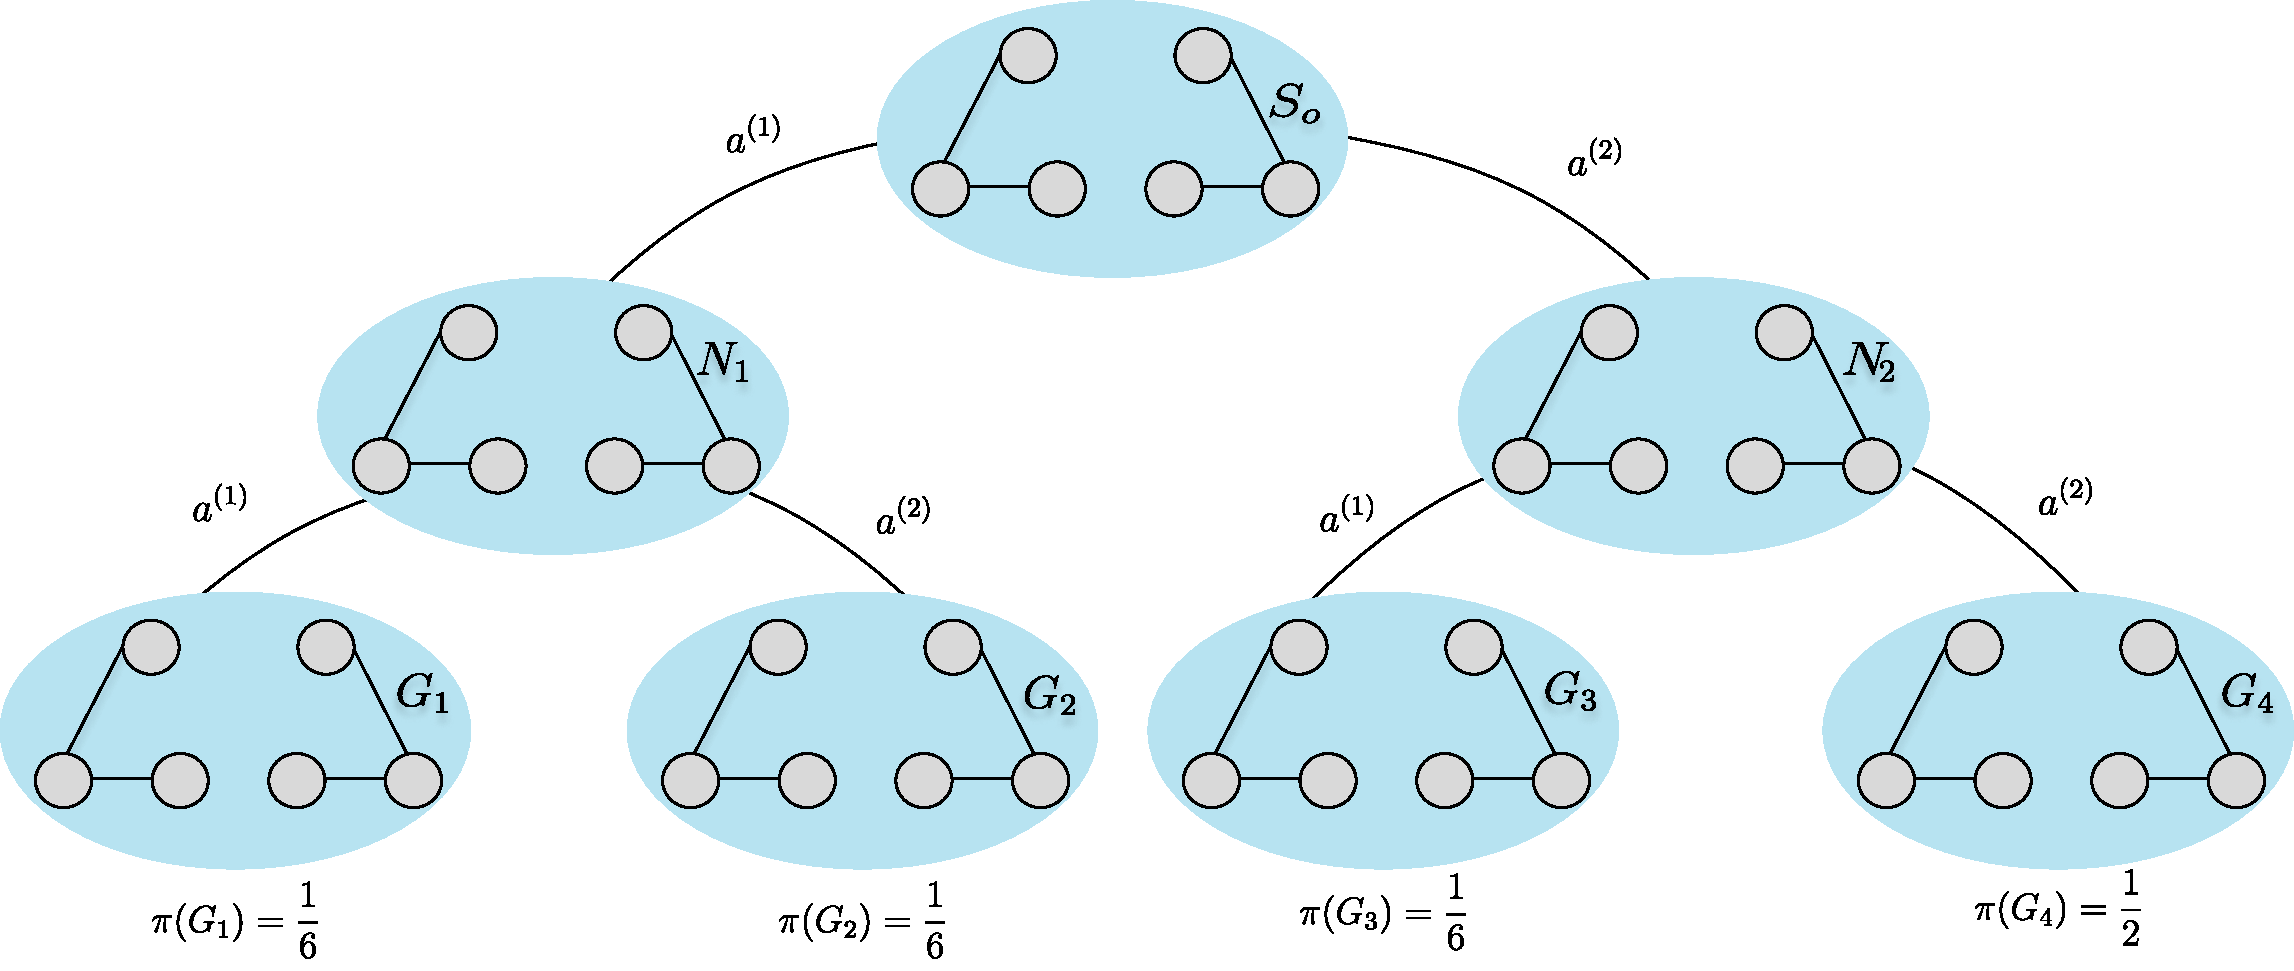
\includegraphics[scale=.3]{gflownets_wl_test.pdf} 
    \caption{A state graph whose downstream distribution is not learnable by a GFlowNet with a policy network is
    parametrized by a 1-WL GNN.} 
    \label{fig:wl_graphs} 
\end{figure}

\begin{theorem}[Distributional constraints of GFlowNets] 
    Let $\mathcal{G} = \{(\mathbf{X}, \mathbf{A}) \colon \mathbf{A} \in \{0,
    1\}^{N \times N}\}$ be the set of equally featured graphs with adjacency matrix $\mathbf{A}$
    and features $\mathbf{r} \in \mathbb{R}^{d}$ ($\mathbf{X} = \mathbf{1}\mathbf{r}^{T} \in \mathbb{R}^{N \times d}$). Let $F_{\theta} \colon \mathcal{G} \rightarrow \Delta_{2}$ be the
    \textit{policy network} that maps a graph $G \in \mathcal{G}$ to a point within the simplex of action-probabilities $\Delta_{2} =
    \{(a^{(1)}, a^{(2)}) \colon a^{(1)} + a^{(2)} = 1 \text{ and
    } a^{(1)}, a^{(2)} \ge 0\}$. See Figure~\ref{fig:wl_graphs}. Suppose that the policy network is parametrized by an 1-WL GNN with parameters $\theta$. Let $\pi$ be a distribution on the
    graphs $\{G_{i} \colon i \in \{1, 2, 3, 4\}\}$ of Figure~\ref{fig:wl_graphs} with $\pi(G_{1}) = \pi(G_{2}) = \pi(G_{3}) =
    \frac{1}{6}$ and $\pi(G_{4}) = \frac{1}{2}$. In these settings, there does not exist a
    $\theta$ such that the downstream distribution induced by the policy network equals $\pi$. 
\end{theorem}

\begin{proof}
    Let $p_{\theta}(X | S_{o})$ be the marginal transition probability learned by the GFlowNet of reaching the state $X
    \in \mathcal{G}$
    through the generative process characterized by the state graph of Figure~\ref{fig:wl_graphs} and the policy network
    $F_{\theta}$. We will show that
    $p_{\theta}(G_{i} | S_{o})$ is -- for any $\theta$ -- necessarily different of $\pi(G_{i})$ for at least two graphs
    in $\pi$'s support. 

    For this, notice that the Markovity of the stochastic transitions learned by the GFlowNet
    entails that 
    $p_{\theta}(G_{1} | S_{o}) = p_{\theta}(N_{1} | S_{o}) p_{\theta}(G_{1} | N_{1})$, 
    $p_{\theta}(G_{2} | S_{o}) = p_{\theta}(N_{1} | S_{o}) p_{\theta}(G_{2} | N_{1})$, 
    $p_{\theta}(G_{3} | S_{o}) = p_{\theta}(N_{2} | S_{o}) p_{\theta}(G_{3} | N_{2})$ and  
    $p_{\theta}(G_{4} | S_{o}) = p_{\theta}(N_{2} | S_{o}) p_{\theta}(G_{4} | N_{2})$. 
    Notably, the indistinguishability of the graphs $N_{1}$ and $N_{2}$ according to the 1-WL 
    isomorphism test implies that $F_{\theta}(N_{1}) = F_{\theta}(N_{2})$ and hence the transition  
    probabilities must satisfy $p_{\theta}(G_{1} | N_{1}) = p_{\theta}(G_{3} | N_{2})$ and $p_{\theta}(G_{2} | N_{1}) =
    p_{\theta}(G_{4} | N_{2})$. 

    Contradictorily, suppose that there is a $\theta$ such that the policy network $F_{\theta}$ is perfectly adjusted to the target distribution $\pi$.
    Hence, $p_{\theta}(G_{i} | S_{o}) = \pi(G_{i})$ for each $i \in \{1, 2, 3, 4\}$. Nonetheless, the representational equivalence of
    $N_{1}$ and $N_{2}$ and the Markovian assumption imply that 

    \begin{equation*} 
        \begin{split} 
        p_{\theta}(N_{1} | S_{o}) = \frac{\pi(G_{1})}{p_{\theta} (G_{1} | N_{1})} 
        = \frac{\pi(G_{3})}{p_{\theta} (G_{3} | N_{2})} = p_{\theta}(N_{2} | S_{o}) 
        \text{ and that } \\ 
        p_{\theta}(N_{1} | S_{o}) = \frac{\pi(G_{2})}{p_{\theta}(G_{2} | N_{1})} \neq 
        \frac{\pi(G_{4})}{p_{\theta}(G_{4} | N_{2})} = p_{\theta}(N_{2} | S_{o}).
        % p_{\theta}(N_{1} | S_{o}) = 
    \end{split} 
    \end{equation*} 

   \noindent This contradiction guarantees that $p(G_{i} | S_{o})$ is necessarily different from $\pi(G_{i})$ for at
   least a pair of graphs and asseverates that the distribution characterized by the state graph of
   Figure~\ref{fig:wl_graphs} is unlearnable by a GFlowNet parametrized by a 1-WL GNN. 
\end{proof}

\begin{remark}
    The previous theorem states the limitations of a GFlowNet parametrized by a 1-WL GNN. The alternative use of a more
    expressive yet not permutationally invariant flow parametrization would entail a factorially large increase of the
    size of the state graph, as equivalent graphs with different labelling would be treated differently by the flow
    estimator, and lead to a computationally untractable problem. The next theorem characterizes a weak relationship
    between the size of the state graph and the statistical efficiency of a maximally entropic exploratory policy within the state graph.   
\end{remark}

\subsubsection*{Author Contributions}
If you'd like to, you may include  a section for author contributions as is done
in many journals. This is optional and at the discretion of the authors.

\subsubsection*{Acknowledgments}
Use unnumbered third level headings for the acknowledgments. All
acknowledgments, including those to funding agencies, go at the end of the paper.
 

% \appendix

% \section{Claimed Emergent Abilities}
% \label{app:claimed_emergent_abilities}

% We compile the models, tasks and metrics that different papers have claimed reveal emergent abilities of large language models. This list may be incomplete or inaccurate, but represents a good faith attempt to compile this information. Note: quantifying model scale when an ability emerges is complicated by the fact that different papers report model scale differently, either as (a) number of parameters \cite{brown2020language, ganguli2022predictability}, (b) effective number of parameters \cite{srivastava2022beyond} or (c) training FLOPs \cite{wei2022emergent}.

% \begin{table}[h!]
%     \centering
%     \begin{tabular}{|l|c|c|c|}
%     \hline
%         Task & Model Families & Metric & Model Scale at Emergence \\
%         \hline
%         2-Digit Addition \cite{brown2020language} & GPT-3 & Accuracy & 13B Parameters\\
%         2-Digit Subtraction \cite{brown2020language} & GPT-3 & Accuracy & 13B Parameters\\
%         3-Digit Addition \cite{brown2020language, ganguli2022predictability} & GPT-3 & Accuracy & 175B Parameters\\
%         3-Digit Subtraction \cite{brown2020language} & GPT-3 & Accuracy & 175B Parameters\\
%         MMLU \cite{ganguli2022predictability} & GPT-3, Gopher & Accuracy & 200B, 300B Parameters\\
%         Program Synthesis \cite{ganguli2022predictability} & Google Internal & \% Samples Solving Task & 200B Parameters\\
%         Figure of Speech Detection \cite{srivastava2022beyond} & ? & ? & $\sim 10^{11}$ Effective Parameters \\
%         IPA Transliterate \cite{srivastava2022beyond, wei2022emergent} & LaMDA, GPT-3 & BLEU & $\sim 10^{23}, \sim 10^{23}$ Training FLOPs\\
%         Periodic Elements \cite{srivastava2022beyond} & ? & ? & ?\\
%         Modified Arithmetic \cite{srivastava2022beyond, wei2022emergent} & GPT-3, LaMDA & Accuracy & $\sim 10^{23}, \sim 10^{24}$ Training FLOPs\\
%         Repeat Copy Logic \cite{srivastava2022beyond} & ? & ? & $10^{11}$ Effective Parameters\\
%         Word Unscrambling \cite{srivastava2022beyond, wei2022emergent} & LaMDA & Exact Match & $\sim 10^{24}$ Training FLOPs\\
%         Persian QA \cite{wei2022emergent} & PaLM & Exact Match & $\sim 10^{24}$ Training FLOPs\\
%         Truthful QA \cite{wei2022emergent} & Gopher & Accuracy & $\sim 10^{23}$ Training FLOPs\\
%         Grounded Mappings \cite{wei2022emergent} & ? & ? & ?\\
%         Multi-task NLU \cite{wei2022emergent} & ? & ? & ?\\
%         Word in context \cite{wei2022emergent} & ? & ? & $\sim 10^{24}$ Training FLOPs\\
%         \hline
%     \end{tabular}
%     \newline
%     \caption{\textbf{Tasks, model families, metrics and number of parameters for emergent abilities.}}
%     \label{tab:my_label}
% \end{table}


% \section{Exponentiated Negative Cross Entropy Lower Bounds Accuracy}
% \label{app:acc_bound}

% Consider batch size $B$ with length $L$. During training i.e. with teacher-forcing, the per-token accuracy (averaged over batch index $b$ and sequence index $l$) is defined as:
% %
% \begin{align}
%     \text{Acc} &\defeq \frac{1}{B} \sum_b \frac{1}{L} \sum_l p(t_{bl}^* | t_{b, <l}^*)\\
%     &= \frac{1}{BL} \sum_{b, l} p(t_{bl}^* | t_{b, <l}^*)
% \end{align}

% The cross entropy (commonly averaged over the batch) is defined as:
% %
% \begin{align}
%     \mathcal{L}_{CE} &\defeq -\frac{1}{B} \sum_b \log p(t_{b 1}^*, ..., t_{b L}^*)\\
%     &= -\frac{1}{B} \sum_b \log \prod_l p(t_{b l}^*| t_{b, <l}^*)\\
%     &= -\frac{1}{B} \sum_{b, l} \log p(t_{bl}^* | t_{b, <l}^*)
% \end{align}

% To make the comparison between accuracy and cross entropy a little easier, let's normalize the cross entropy by the sequence length:
% %
% \begin{align}
%     \mathcal{L}_{CE/L} &\defeq \frac{1}{L}\mathcal{L}_{CE}\\
%     &=  -\frac{1}{BL} \sum_{b, l} \log p(t_{bl}^* | t_{b, <l}^*)
% \end{align}

% Recall that Jensen's inequality tells us that for any random variable $X$, $\log \mathbb{E}[X] \geq \mathbb{E}[\log X]$. The relationship between sequence-length-normalized cross entropy and accuracy is thus:
% %
% \begin{align}
%     -\mathcal{L}_{CE/L} = \frac{1}{BL} \sum_{b, l} \log p(t_{bl}^* | t_{b <l}^*) &\leq \log \frac{1}{BL} \sum_{b, l}  p(t_{bl}^* | t_{b <l}^*) = \log \text{Acc}\\
%     \exp(- \mathcal{L}_{CE/L}) &\leq \text{Acc}
% \end{align}

% Consequently, we see that driving the cross entropy loss to $0$ necessarily drives the accuracy to $1$.

% TODO: Can we use the second moment method to derive bounds on how (un)likely a subset of tokens are to deviate from the mean?


\section{Approximate Behavior of Metrics on Sequential Data}
\label{app:metric_scaling}

How do different metrics behave when used to measure autoregressive model outputs? Precisely answering this question is tricky and possibly analytically unsolvable, so we provide an approximate answer here.

Notationally, we consider $N$ test data of length $L$ (here, length is measured in tokens) with targets denoted $t_n \defeq (t_{n1}, t_{n2}, ... t_{nL})$, the autoregressive model has a true-but-unknown per-token error probability of $\epsilon \in [0, 1]$ and the model outputs prediction $\hat{t}_n \defeq (\hat{t}_{n1}, \hat{t}_{n2}, ... \hat{t}_{nL})$. This assumes that the model's per-token error probability is constant, which is empirically false, but modeling the complex dependencies of errors is beyond our scope.

\subsection{Per-Token Error Probability is Resolution-Limited}
\label{app:metric_scaling:resolution_limited}

Note that because we have $N$ test data, each of length $L$, our resolution for viewing the per-token error probability $\epsilon$ is limited by $1/NL$. 
Here, resolution refers to ``the smallest interval measurable by a scientific instrument; the resolving power."
To explain what resolution means via an example, suppose one wants to measure a coin's probability of yielding heads.
After a single coin flip, only two outcomes are possible (H, T), so the resolution-limited probability of heads is either $0$ or $1$.
After two coin flips, four outcomes are possible (HH, HT, TH, TT), so the resolution-limited probability of heads is now one of $0, 0.5, 1$.
After $F$ coin flips, we can only resolve the coin's probability of yielding heads up to $1/F$.
Consequently, we introduce a resolution-limited notation:
%
\begin{equation}
    \nint{a}_b \defeq \text{$a$ rounded to the nearest integer multiple of $1/b$}
\end{equation}

\subsection{Token Edit Distance}
\label{app:metric_scaling:token_edit_distance}

We first consider an adaptation of the Levenshtein (string edit) distance for models that function on tokens rather than characters, an adaptation we term the \textit{token edit distance}. The token edit distance between two token sequences $t_n, \hat{t_n}$ is defined as the integer number of additions, deletions or substitutions necessary to transform $t_n$ into $\hat{t}_n$ (or vice versa).

\begin{align}
    \text{Token Edit Distance}(t_n, \hat{t}_n)  &\defeq \text{Num Substitutions} + \text{Num. Additions} + \text{Num. Deletions}\\
    &= \sum_{\ell =1}^L \mathbb{I}[t_{n\ell} \neq \hat{t}_{n\ell}] + \text{Num. Additions} + \text{Num. Deletions}\\
    &\geq \sum_{\ell =1}^L \mathbb{I}[t_{n\ell} \neq \hat{t}_{n\ell}]
\end{align}

The expected token edit distance is therefore:

\begin{align}
    \mathbb{E}[\text{Token Edit Distance}(t_n, \hat{t}_n)] &\geq \mathbb{E}[\sum_{\ell =1}^L \mathbb{I}[t_{n\ell} \neq \hat{t}_{n\ell}]]\\
    &= \sum_{\ell =1}^L p(t_{n\ell} \neq \hat{t}_{n\ell})\\
    &\approx L (1 - \epsilon)
\end{align}

The resolution-limited expected token edit distance is therefore:

\begin{equation}
    \nint{\mathbb{E}[\text{Token Edit Distance}(t_n, \hat{t}_n)]}_{NL} \geq L \Big(1 - \nint{\epsilon}_{NL} \Big)
\end{equation}

From this, we see that the expected token edit distance scales approximately linearly with the resolution-limited per-token probability. The real rate is slightly higher than linear because additions and deletions contribute an additional non-negative cost, but modeling this requires a model of how likely the model is to overproduce or underproduce tokens, which is something we do not currently possess.

\subsection{Accuracy}
\label{app:metric_scaling:accuracy}

\begin{align}
    \text{Accuracy}(t_n, \hat{t}_n) &\defeq \mathbb{I}[\text{No additions}] \, \mathbb{I}[\text{No deletions}] \, \prod_{l=1}^L \mathbb{I}[t_{nl} = \hat{t}_{nl}]\\
    &\approx \prod_{l=1}^L \mathbb{I}[t_{nl} = \hat{t}_{nl}]
\end{align}

As with the Token Edit Distance (App. \ref{app:metric_scaling:accuracy}), we ignore how likely the language model is to overproduce or underproduce tokens because we do not have a good model of this process. Continuing along,

\begin{align}
    \mathbb{E}[\log \text{Accuracy}] &= \sum_l \mathbb{E}[\log \mathbb{I}[t_{nl} = \hat{t}_{nl}]]\\
    &\leq \sum_l \log \mathbb{E}[\mathbb{I}[t_{nl} = \hat{t}_{nl}]]\\
    &\approx L \log (1- \epsilon)
    % \exp(\mathbb{E}[\log \text{Accuracy}]) &= \exp (\sum_l \mathbb{E}[\log \mathbb{I}(t_{nl}, \hat{t}_{nl})])\\
    % &=
\end{align}

Taking an approximation that would make most mathematicians cry:

\begin{align}
    \mathbb{E}[\text{Accuracy}] &\approx \exp(\mathbb{E}[\log \text{Accuracy}])\\
    &= (1 - \epsilon)^L\\
\end{align}

This reveals that accuracy \textbf{approximately} falls geometrically with target token length. The resolution-limited expected accuracy is therefore:

\begin{equation}
    \nint{\mathbb{E}[\text{Accuracy}]}_{NL} = \nint{(1 - \epsilon)^L}_{NL}
\end{equation}

From this we can see that choosing a nonlinear metric like Accuracy is affected significantly more by limited resolution because Accuracy forces one to distinguish quantities that decay rapidly.

\subsection{ROUGE-L-Sum}
\label{app:metric_scaling:rougeLsum}

\begin{figure}
    \centering
    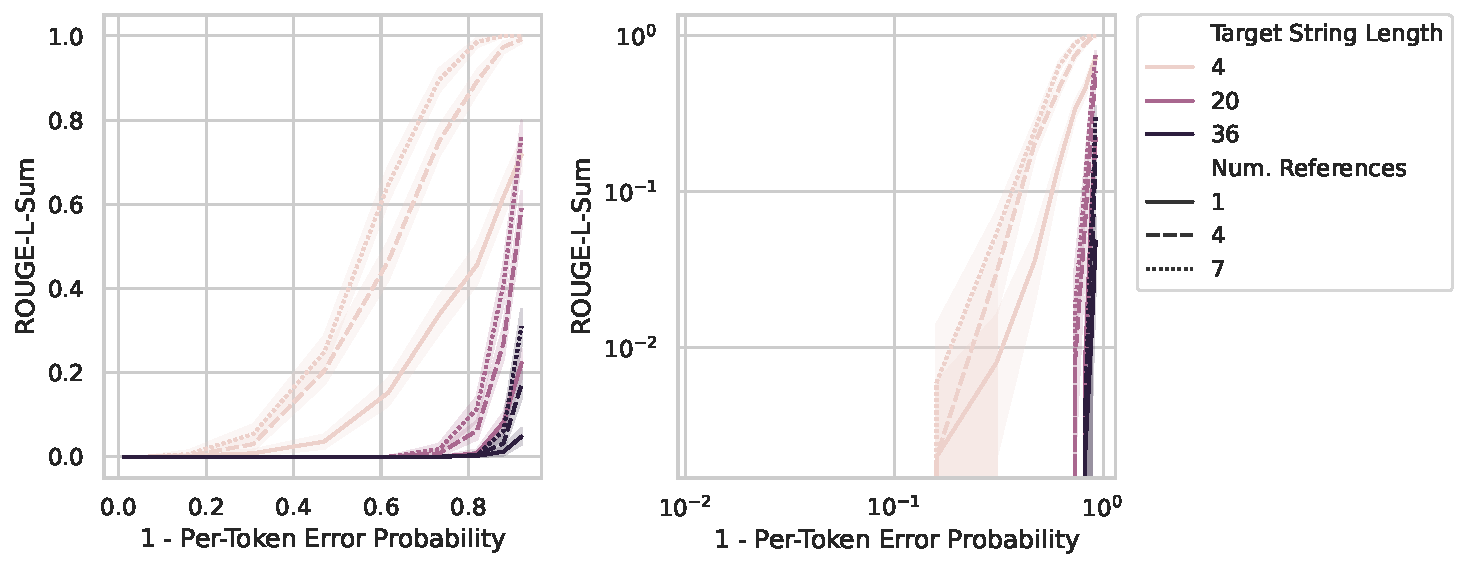
\includegraphics[width=0.95\textwidth]{figures/rouge_understanding/rougeLsum_vs_token_error_prob_scaling_simulation.pdf}
    \caption{\textbf{ROUGE-L-Sum is a sharp metric.} Simulations show that as the per-token error probability slightly increase (e.g. from 0.05 to 0.1), the ROUGE-L-Sum metric sharply falls.}
    \label{fig:app:metric_scaling:rougeLsum}
\end{figure}


Another BIG-Bench metric \cite{srivastava2022beyond} is ROUGE-L-Sum \cite{lin2004rouge}, a metric based on the longest common subsequence (LCS) between two sequences. Section 3.2 of \cite{lin2004rouge} gives the exact definition, but the key property is that ROUGE-L-Sum measures the ``union" LCS, which means ``stitching" together LCSs across the candidate and multiple references. As explained in the original paper: if the candidate sequence is $c = w_1 w_2 w_3 w_4 w_5$, and if there are two reference sequences $r_1 = w_1 w_2 w_6 w_7 w_8$ and $r_2 = w_1 w_3 w_8 w_9 w_5$, then $LCS(r_1, c) = w_1 w_2$ and $LCS(r_2, c) =w_1 w_3 w_5$, then the \textit{union} 
-LCS of $c, r_1, r_2$ is $w_1 w_2 w_3 w_5$, with length 4. Intuitively, this disproportionately benefits models with smaller error rates because their mistakes can be ``stitched" across multiple references; this is confirmed in simulation (Fig. \ref{fig:app:metric_scaling:rougeLsum}).


% \subsection{BLEU}
% \label{app:metric_scaling:bleu}


% \subsection{Emergence does not require on scaling laws: decreasing cross-entropy loss and stricter exact match is all you need }

% The goal of this section is to show that scaling laws are not necessary to create emergence and that many functional forms of the loss are valid as long as the form decreases as some other variable decreases -- say the number of parameters in the model.
% This typically holds in modern machine learning. 
% We do this by considering different functional forms of the cross entropy $CE(N)$, as a function of the number of parameters $N$, and show emergence, i.e. sharpness and unpredictability.
% We illustrate this by showing the programmer can exaggerate the sharpness (and therefore emergence) by implying increasing the exact number of tokens required to get correct in the accuracy, i.e. increasing $L$ in our notation.

% \subsubsection{Argument}

% Recall from section \ref{sec:alt_explanation} the accuracy requiring all $L$ tokens to be correct for a model of size $N$ as a function of cross-entropy $CE(N)$:

% \begin{equation*}
%     \text{Accuracy}(N) \approx p_N(\text{single token correct})^{\text{num. of tokens}} = \exp \Big(- CE(N) \Big)^L
% \end{equation*}

% We plot this equation using three functional forms for a decreasing cross-entropy loss in figure \ref{fig:decreasing_loss_leads_to_emergence_as_L_increases} for increasing values of $L$.
% These increasing values of $L$ induce a sharper -- therefore, seemingly more emergent curve when plotting the accuracy. 
% This means that if the programmer simply requires a stricter accuracy, he can make a perfectly smooth and predictable cross-entropy loss suddenly become sharp and unpredictable, i.e. ``emergent". 
% We show numerically it is independent of the functional form and instead that it only requires the cross-entropy to be decreasing and the accuracy metric to have some non-linear transformation that makes it sharper. 
% Therefore, if one had only tracked the cross-entropy loss instead, one could have had a smooth predictable curve for the models.
% This implies small-scale experimentation is still relevant, and we wish to highly that GPT-4 \cite{gpt4} small-scale experiment in conjunction with scaling loss. 
% We'd like to emphasize that changing the evaluation metric can suddenly induce emergence, and it is not an intrinsic property of the model. 

% %The goal will be to show that if $CE(N)$ decreases with different functional forms that $acc$ is emergent (either sharp or unpredictable).
% % TODO: sharp due to L
% % TODO: unpredictable due to constant and L

% \begin{figure}[htbp]
%   \centering
%   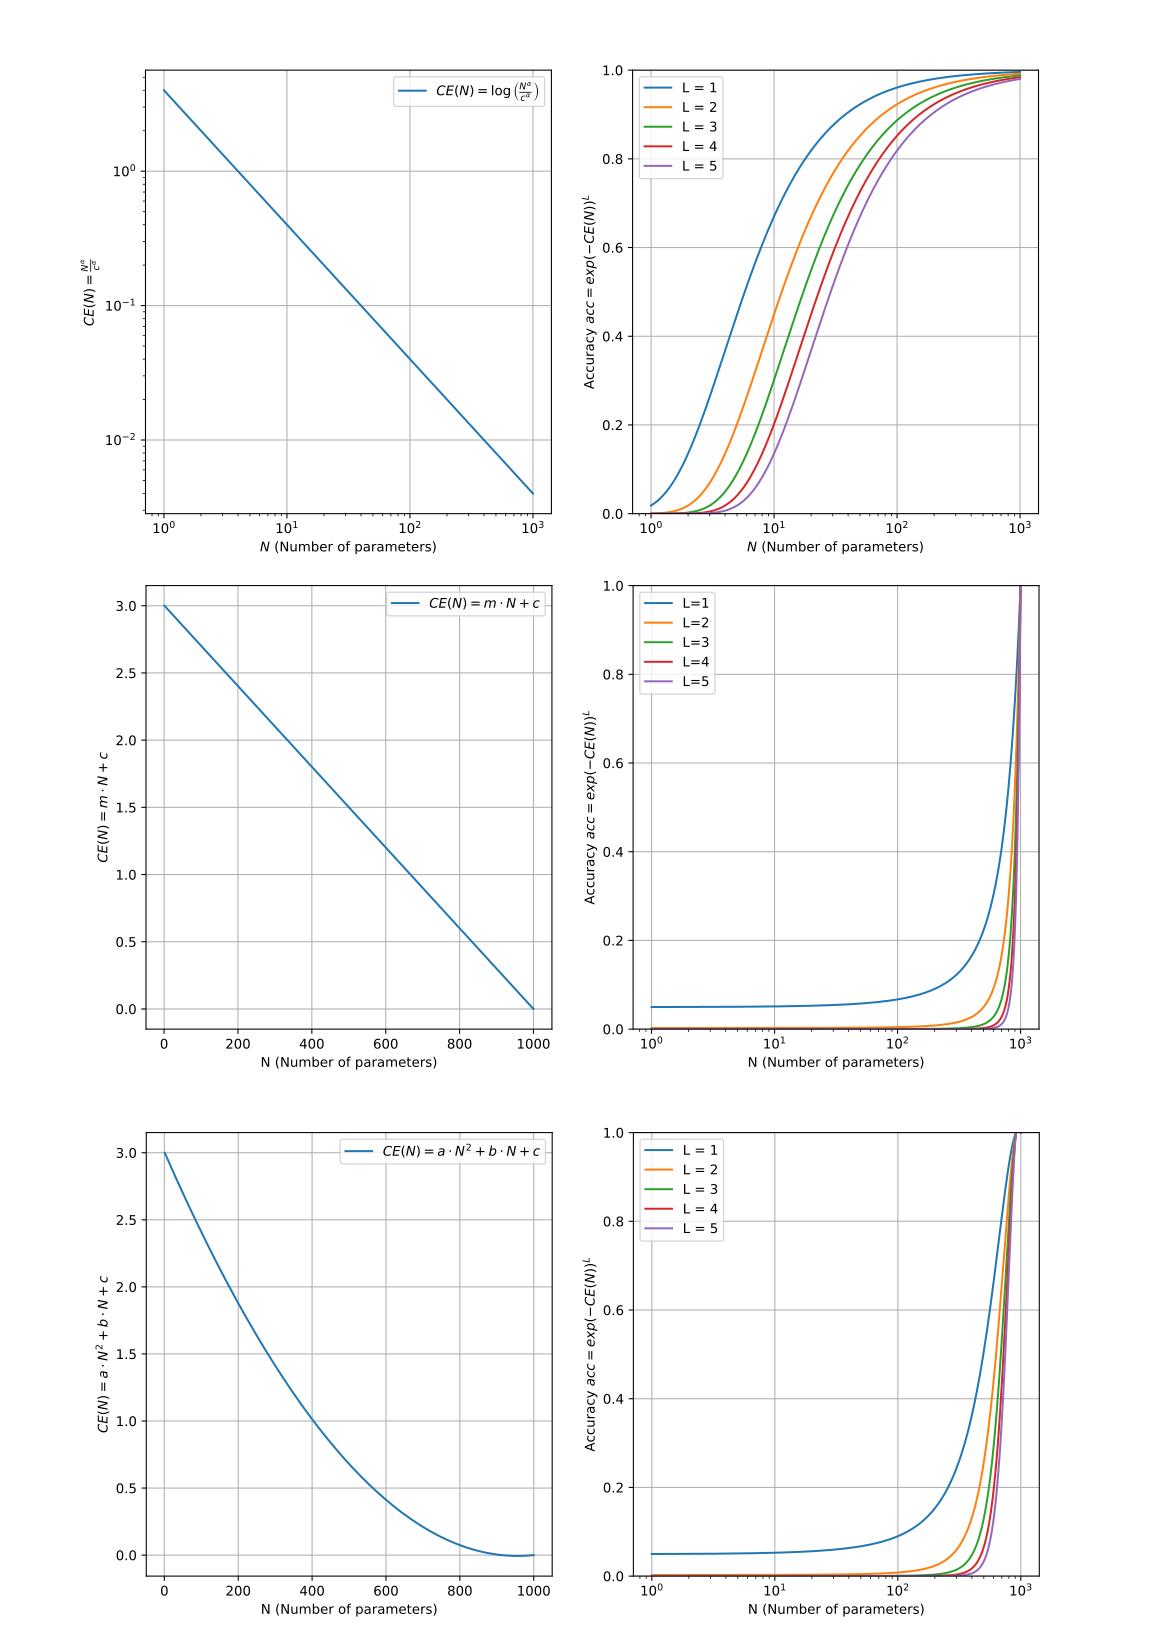
\includegraphics[width=0.8\textwidth]{figures/loss_decreasing_leads_to_emergence/decreasing_loss_leads_to_emergence_as_L_increases.png}
%   \caption{
%   \textbf{Emergence does not depend on scaling laws: any decreasing cross-entropy loss induces apparent emergence as L increases as you require more tokens to be exactly correct, i.e. L increases.}
%   The first row shows the same argument as in the main section, where a decreasing cross-entropy loss as a scaling law induces emergence as $L$ increases.
%   The second row shows the that apparent emergence is induced even when the cross-entropy loss decreases linearly.
%   The third row shows that the apparent emergence is induced when the cross-entropy loss decreases quadratically.
%   Emergence is amplified in this case especially by the increase in sharpness as more tokens are required to be correct. 
%   This means that simply changing the evaluation metric can suddenly induce emergence, and it is not an intrinsic property of the model. 
%   }
%   \label{fig:decreasing_loss_leads_to_emergence_as_L_increases}
% \end{figure}


\section{Inducing Emergent Abilities in Networks on Vision Tasks}
\label{app:sec:inducing_emergence_vision}

\subsection{Emergent Classification of MNIST Handwritten Digits by Convolutional Networks}

\begin{figure}
    \centering
    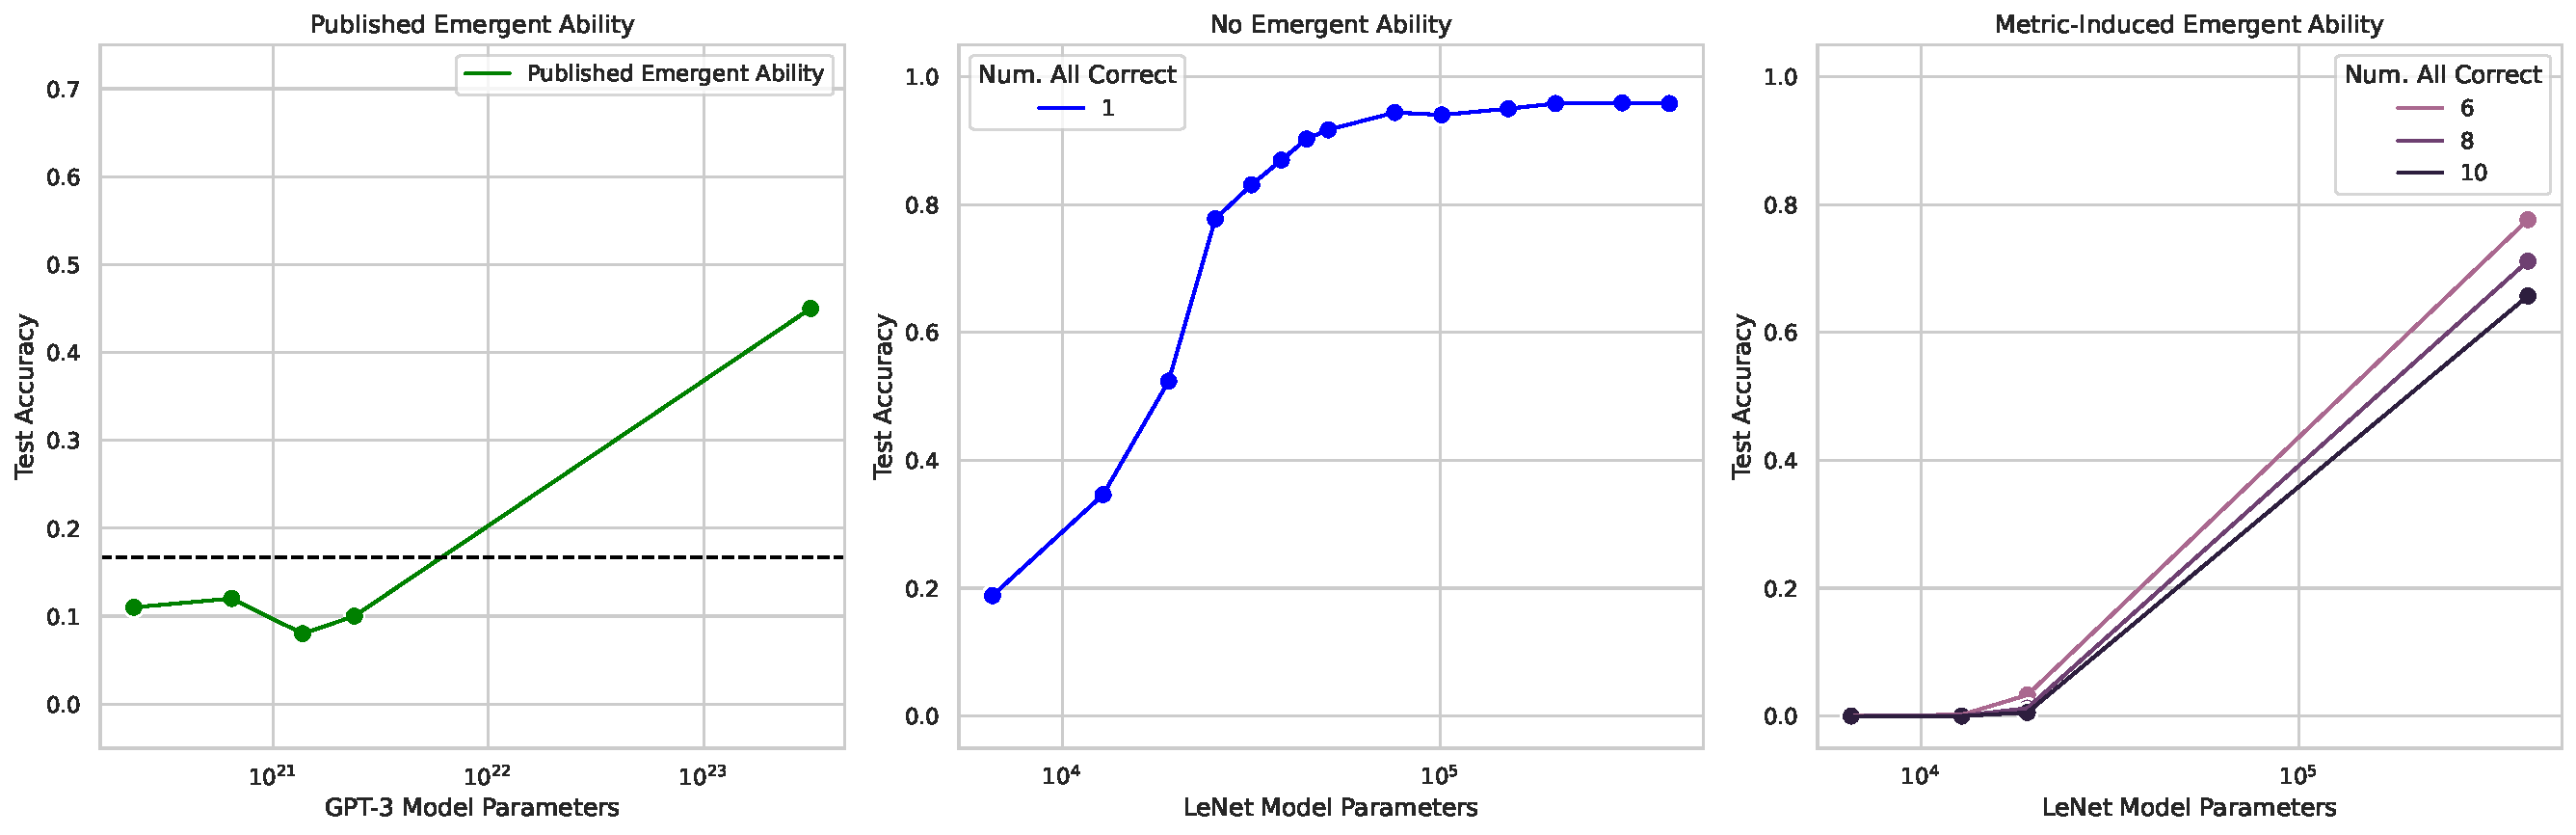
\includegraphics[width=\textwidth]{figures/vision/no_emergence_and_emergence_dataset=mnist.pdf}
    \caption{\textbf{Induced emergent MNIST classification ability in convolutional networks.} (A) A published emergent ability from the BIG-Bench Grounded Mappings task \cite{wei2022emergent}. (B) LeNet trained on MNIST \cite{lecun1998mnist} displays a predictable, commonplace sigmoidal increase in test accuracy as model parameters increase. (C) When accuracy is redefined as correctly classifying $K$ out of $K$ independent test data, this newly defined metric induces a seemingly unpredictable change.}
    \label{fig:vision_mnist}
\end{figure}

We begin by inducing an emergent classification ability in a LeNet convolutional neural network family \cite{lecun1998gradient}, trained on the MNIST handwritten digits dataset \cite{lecun1998mnist}.
This family displays smoothly increasing test accuracy as the number of parameters increase (Fig. \ref{fig:vision_mnist}B).
To emulate the accuracy metric used by emergence papers \cite{ganguli2022predictability, wei2022emergent, srivastava2022beyond}, we use \textit{subset accuracy}: 1 if the network classifies $K$ out of $K$ (independent) test data correctly, 0 otherwise.
Under this definition of accuracy, the model family displays an ``emergent" ability to correctly classify sets of MNIST digits as $K$ increases from $1$ to $5$, especially when combined with sparse sampling of model sizes (Fig. \ref{fig:vision_mnist}C).
This convolutional family's emergent classification ability qualitatively matches published emergent abilities, e.g., at the BIG-Bench Grounded Mappings task \cite{wei2022emergent} (Fig. \ref{fig:vision_mnist}A).
 

\section{Training of SB-GFlowNets} 

\begin{algorithm}[!t] 
\caption{Training a SB-GFlowNet by minimizing $\mathcal{L}_{SB}$}\label{alg:cap}
\label{alg:training} 
\begin{algorithmic}
\Require $\left(\mathcal{D}_{t}\right)_{T \ge t \ge 1}$ streaming data sets, $f(\cdot | x)$ a likelihood model parametrized by $x$, $\pi(x)$ a prior distribution over $\mathcal{X}$ 
\Ensure $G_{T}$ samples proportionally to $\left( \prod_{t=1}^{T} f(\mathcal{D}_{t} | x) \right) \pi(x)$ 
% \State $\log Z_{1} \gets \log \mathbb{E}_{p_{F}}\left[ \nicefrac{\tilde{\pi}(x)}{p_{F}(\tau)}\right]$ \Comment Initialize $\log Z_{1}$  
\State $G_{1} \gets\! (p_{F}^{1}, p_{B}^{1}, Z_{1}) \coloneqq \underset{p_{F}, p_{B}, Z}{\argmin}\, 
\mathbb{E}_{\tau \sim \xi} \left[ \mathcal{L}_{TB}(\tau ; p_{F}, p_{B}, Z)\right]$ \Comment{Roughly minimize $\mathcal{L}_{TB}$ via SGD} 

\For{$t$ in $\{2, \dots, T\}$} 
    % \State $\log Z_{t} \gets \log Z_{t - 1} + \!\!\!\! \underset{x \sim p_{\top}^{(t - 1)}} {\mathbb{E}} \left[ f(\mathcal{D}_{t} | x) \right]$ \Comment Initialize $\log Z_{t}$   
    \Comment{Roughly minimize $\mathcal{L}_{SB}$ via SGD}
    \State $G_{t} \gets (p_{F}^{(t)}, p_{B}^{(t)}, Z_{t}) \coloneqq\underset{p_{F}, p_{B}, Z}{\argmin} \ \mathbb{E}_{\tau \sim p_{\top}^{(t - 1)}} \left[ \mathcal{L}_{SB}(\tau ; p_{F}, p_{B}, Z; G_{t - 1}) \right]$  
\EndFor 
% $(p_{F}^{(1)}, p_{B}^{(1)}, Z_{1}) = \argmin $
\end{algorithmic}
\end{algorithm}

\autoref{alg:training} outlines the training of a SB-GFlowNet by minimizing the SB loss. As we described in the text, the first GFlowNet is trained conventionally by approximately minimizing either the TB loss or the KL divergence between the forward and backward policies. Then, the subsequent models are trained by the approximate minimization of either the SB loss or streaming balance criterion. Notably, the problem of streaming update may be framed as the learning of GFlowNets with stochastic rewards \cite{stochastic}, which are not determistically associated to the terminal states.  

\section{Proofs} 
\label{sec:app:proofs}
\subsection{Proof of \autoref{prop:streaming}} 

We are assuming that $p_{\top}^{(t)}  \propto \pi_{t}$ and that $\mathbb{E}_{\tau \sim \xi}[\mathcal{L}_{SB}(\tau)] = 0$ for a distribution $\xi$ of full support. Thus, $\mathcal{L}_{SB}(\tau) = 0$ for all $\tau$. As a consequence,
\begin{equation}
    p_{F}^{(t + 1)}(\tau) = \left( \frac{p_{B}^{(t + 1)}(\tau | x)}{p_{B}^{(t)}(\tau | x)}  \right) \cdot \frac{Z_{t}}{Z_{t+1}} \cdot  p_{F}^{(t)}(\tau) f(\mathcal{D}_{t + 1} | x). 
\end{equation}
By assumption, $(p_{F}^{(t)}, p_{B}^{(t)}, Z_{t})$ satisfy the trajectory balance condition with respect to $\pi_{t}$, therefore, $Z_t\cdot p_F^{(t)}(\tau) = p_B^{(t)}(\tau|x)\pi_t(x)$. Thus, 
\begin{equation}
    \frac{p_{F}^{(t + 1)}(\tau)}{p_{B}^{(t + 1)}(\tau | x)} = Z_{t + 1} \pi_{t}(x) f(\mathcal{D}_{t + 1} | x).
\end{equation}
Finally, by summing over $\tau \rightsquigarrow x$:
\begin{align}
    p_{\top}^{(t + 1)}(x)
    &\coloneqq \mathbb{E}_{\tau \sim p_{B}^{(t + 1)}(\cdot | x)}\left[\frac{p_{F}^{(t + 1)}(\tau)}{p_{B}^{(t + 1)}(\tau | x)}\right]
    \propto \pi_{t}(x) f(\mathcal{D}_{t + 1} | x)\\
    &\propto \pi_{t + 1}(x).
\end{align}

\subsection{Proof of \autoref{prop:a}} 

Firstly, we note that $\delta_{LS}^{\xi}(p, q)$ is a metric. Thus, by the triangle inequality, 
\begin{equation} \label{eq:app:aa} 
    \delta_{LS}^{\pi_{t + 1}}\left(p_{\top}^{(t + 1)}, \pi_{t + 1}\right) \le \delta_{LS}^{\pi_{t + 1}}\left(p_{\top}^{(t + 1)}, \hat{p}_{\top}^{(t + 1)}\right) + \delta_{LS}^{\pi_{t + 1}}\left(\hat{p}_{\top}^{(t + 1)}, \pi_{t + 1} \right).  
\end{equation}
The first term of the right-hand-side of the preceding equation corresponds to the estimation error associated to the GFlowNet's learning problem. For the second term, note that $\hat{p}_{\top}^{(t + 1)}(x) = \frac{Z_{t}}{\hat{Z}_{t + 1}} p_{\top}^{(t)}(x) f(\mathcal{D}_{ t + 1 } | x)$ by assumption ($\hat{p}_{\top}^{(t + 1)}$ satisfies the SB condition). Thus, 
\begin{equation*}
    \begin{aligned} 
        \log \hat{p}_{\top}^{(t + 1)}(x) - \log \pi_{t + 1}(x) &= \log \frac{Z_{t}}{\hat{Z}_{t + 1}} + \log p_{\top}^{(t)}(x) f(\mathcal{D}_{t + 1}|x) -  \log \frac{Z_{t}^{\star}\pi_{t}(x)}{Z_{t + 1}^{\star}} f(\mathcal{D}_{t + 1} | x) \\ 
        &= \log \frac{Z_{t + 1}^{\star}}{\hat{Z}_{t + 1}} + \log \frac{Z_{t}}{Z_{t}^{\star}} + \log \frac{p_{\top}^{(t)}(x)}{\pi_{t}(x)}. % , 
    \end{aligned} 
\end{equation*}
The result follows by a further application of the triangle inequality to $\delta_{LS}^{\pi_{t + 1}}\left(p_{\top}^{(t + 1), \star}, \pi_{t + 1}\right)$, namely, \looseness=-1 
\begin{equation} \label{eq:app:aaa} 
    \begin{aligned} 
        \delta_{LS}^{\pi_{t + 1}}\left(\hat{p}_{\top}^{(t + 1)}, \pi_{t + 1}\right) &= \mathbb{E}_{x \sim \pi_{t + 1}} \left[ \left( \log \frac{Z_{t + 1}^{\star}}{\hat{Z}_{t + 1}} + \log \frac{Z_{t}}{Z_{t}^{\star}} + \log \frac{p_{\top}^{(t)}(x)}{\pi_{t}(x)}  \right)^{2} \right]^{1/2} \\ 
        &\le \left| \log \frac{\hat{Z}_{t + 1}}{Z_{t + 1}^{\star}} \right| + \left| \log \frac{Z_{t}}{Z_{t}^{\star}}\right| + \delta_{LS}^{\pi_{t + 1}}\left(p_{\top}^{(t)}, \pi_{t}\right). 
    \end{aligned} 
\end{equation}
% . 
\autoref{prop:a} is obtained by plugging \autoref{eq:app:aaa} into \autoref{eq:app:aa}. 

% There is a slight difference between the statement and this; should check in later 

\subsection{Proof of \autoref{prop:aa}} 

This result, which follows from reasoning similar to the one in \autoref{prop:a} above, aims to show the dependence of the model's performance on the newly observed dataset. In this sense, notice that \looseness=-1 
\begin{equation} \label{eq:app:A} 
    TV\left(p_{\top}^{(t + 1)}, \pi_{t + 1}\right) \le TV\left(p_{\top}^{(t + 1)}, \hat{p}_{\top}^{(t + 1)} \right) + TV\left(\hat{p}_{\top}^{(t + 1)}, \pi_{t + 1}\right).  
\end{equation}
Thus, since $\hat{p}_{\top}^{(t + 1)}(x) = \frac{Z_{t}}{\hat{Z}_{t + 1}} p_{\top}^{(t)}(x) f(\mathcal{D}_{t + 1} | x)$, 
\begin{equation} \label{eq:app:AA}
    \begin{aligned} 
        TV\left(\hat{p}_{\top}^{(t + 1)}, \pi_{t}\right) &= \frac{1}{2} \sum_{x \in \mathcal{X}} \left|p_{\top}^{(t + 1)}(x) - \pi_{t + 1}(x)\right| \\ 
        &= \frac{1}{2} \sum_{x \in \mathcal{X}} f(\mathcal{D}_{t + 1} | x) \left|\frac{Z_{t}}{\hat{Z}_{t + 1}} p_{\top}^{(t)}(x) - \frac{Z_{t}^{\star}}{Z_{t + 1}^{\star}} \pi_{t}(x)\right| \\ 
        &\le \frac{1}{2} f(\mathcal{D}_{t + 1} | \hat{x}) \sum_{x \in \mathcal{X}} \left| \frac{Z_{t}}{\hat{Z}_{t + 1}} p_{\top}^{(t)}(x) - \frac{Z_{t}^{\star}}{Z_{t + 1}^{\star}} \pi_{t}(x) \right|. 
    \end{aligned} 
\end{equation}
The result follows by plugging \autoref{eq:app:AA} into \autoref{eq:app:A}. 

\subsection{Proof of \autoref{prop:aaa}} 

This result follows from the successive application of the triangle, Pinsker`s \cite{csiszar2011information} and Jensen's inequality applied to the KL divergence. More specifically, first note that the optimal distribution under the KL streaming criterion satisfies $\hat{p}_{\top}^{(t + 1)} \propto p_{\top}^{(t)} f(\mathcal{D}_{t + 1} | x)$. Then, by the triangle inequality, 
\begin{equation} \label{eq:Aa} 
     TV\left(p_{\top}^{(t + 1)}, \pi_{t + 1}\right) \le  TV\left(p_{\top}^{(t + 1)}, \hat{p}_{\top}^{(t +1)} \right) +  TV\left(\hat{p}_{\top}^{(t + 1)}, \pi_{t + 1}\right).    
\end{equation}
For the first term, note that 
\begin{equation} \label{eq:AAAAAAAAA} 
    TV\left(p_{\top}^{(t + 1)}, \hat{p}_{\top}^{(t +1)} \right) \le \frac{1}{2} \sqrt{ \mathcal{D}_{KL}\left[p_{\top}^{(t + 1)} || \hat{p}_{\top}^{(t +1)} \right]} \le \frac{1}{2} \sqrt{\mathcal{D}_{KL} \left[ p_{F}^{(t + 1)} || p\right]}, 
\end{equation}
since $\hat{p}_{F}^{(t + 1)} \propto p$ by definition; recall that $p(\tau) = p_{F}^{(t)}(\tau) f(\mathcal{D}_{t +  1} |x)$. Here, the first inequality follows from Pinsker's inequality and the second one, from the data-processing inequality. For the second term, note that 
\begin{equation} \label{eq:AAa} 
    \hat{p}_{\top}^{(t + 1)}(x) = \frac{p_{\top}^{(t)}(x) f(\mathcal{D}_{t + 1} | x)}{\sum_{y \in \mathcal{X}} p_{\top}^{(t)}(y) f(\mathcal{D}_{t + 1} | y)} = \frac{p_{\top}^{(t)}(x) f(\mathcal{D}_{t + 1} | x)}{\mathbb{E}_{y \in p_{\top}^{(t)}} \left[ f(\mathcal{D}_{t + 1} | x) \right]}, % . 
\end{equation}
with a corresponding representation of $\pi_{t + 1}$ as a function of $\pi_{t}$ and $f(\mathcal{D}_{t + 1} | x)$. The result follows by pluggin~\autoref{eq:AAa} and~\autoref{eq:AAAAAAAAA} into \autoref{eq:Aa}. 

% \subsection{Proof of \autoref{prop:sda}} 

% Firstly, we recall the formalism of the Streaming, Distributed, Asynchronous Bayesian updating framework of \citet{Broderick13}. There, the authors considered the problem of updating a posterior $p(\theta | \mathbf{Y}_{1}, \dots, \mathbf{Y}_{b - 1})$ given a newly observed batch of data $\mathbf{Y}_{b}$ and an approximation $q_{b - 1}$ to $p$. By recursively applying approximation algorithm $\mathcal{A}$ such that $q_{b} = \mathcal{A}(q_{b - 1}, \mathbf{Y}_{b})$ is a good approximation to $p(\cdot | \mathbf{Y}_{1}, \dots, \mathbf{Y}_{b})$ among a family of tractable distributions $\mathcal{Q}$, \citet{Broderick13}'s could obtain accurate approximations to the posterior in a streaming setting. In this context, by taking $\mathcal{Q}$ as the family of distributions learnable by a fixed-architecture GFlowNet and $\mathcal{A}$ as either the KL- or log-squared-violation-minimizing algorithm outlined, e.g., in \autoref{alg:training}, one obtains a SB-GFlowNet as an instantiation of SDA-Bayes. 

\section{Experimental details} \label{sec:app:experiments} 

We provide below details for reproducing our experiments for each considered generative task. To approximately solve the optimization problem outlined in \autoref{alg:training}, we employed the Adam optimizer \cite{kingma2014adam} with a learning rate of $10^{-3}$ for the $p_{F}$'s parameters and $10^{-1}$ for $\log Z_{t}$, following recommendations from \cite{malkin2022trajectory}. Also, we linearly decreased the learning rate during training. Experiments were run in a cluster equipped with A100 and V100 GPUs, using a single GPU per run.  


\subsection{Set generation} 

\begin{figure}[h!]
    \centering
    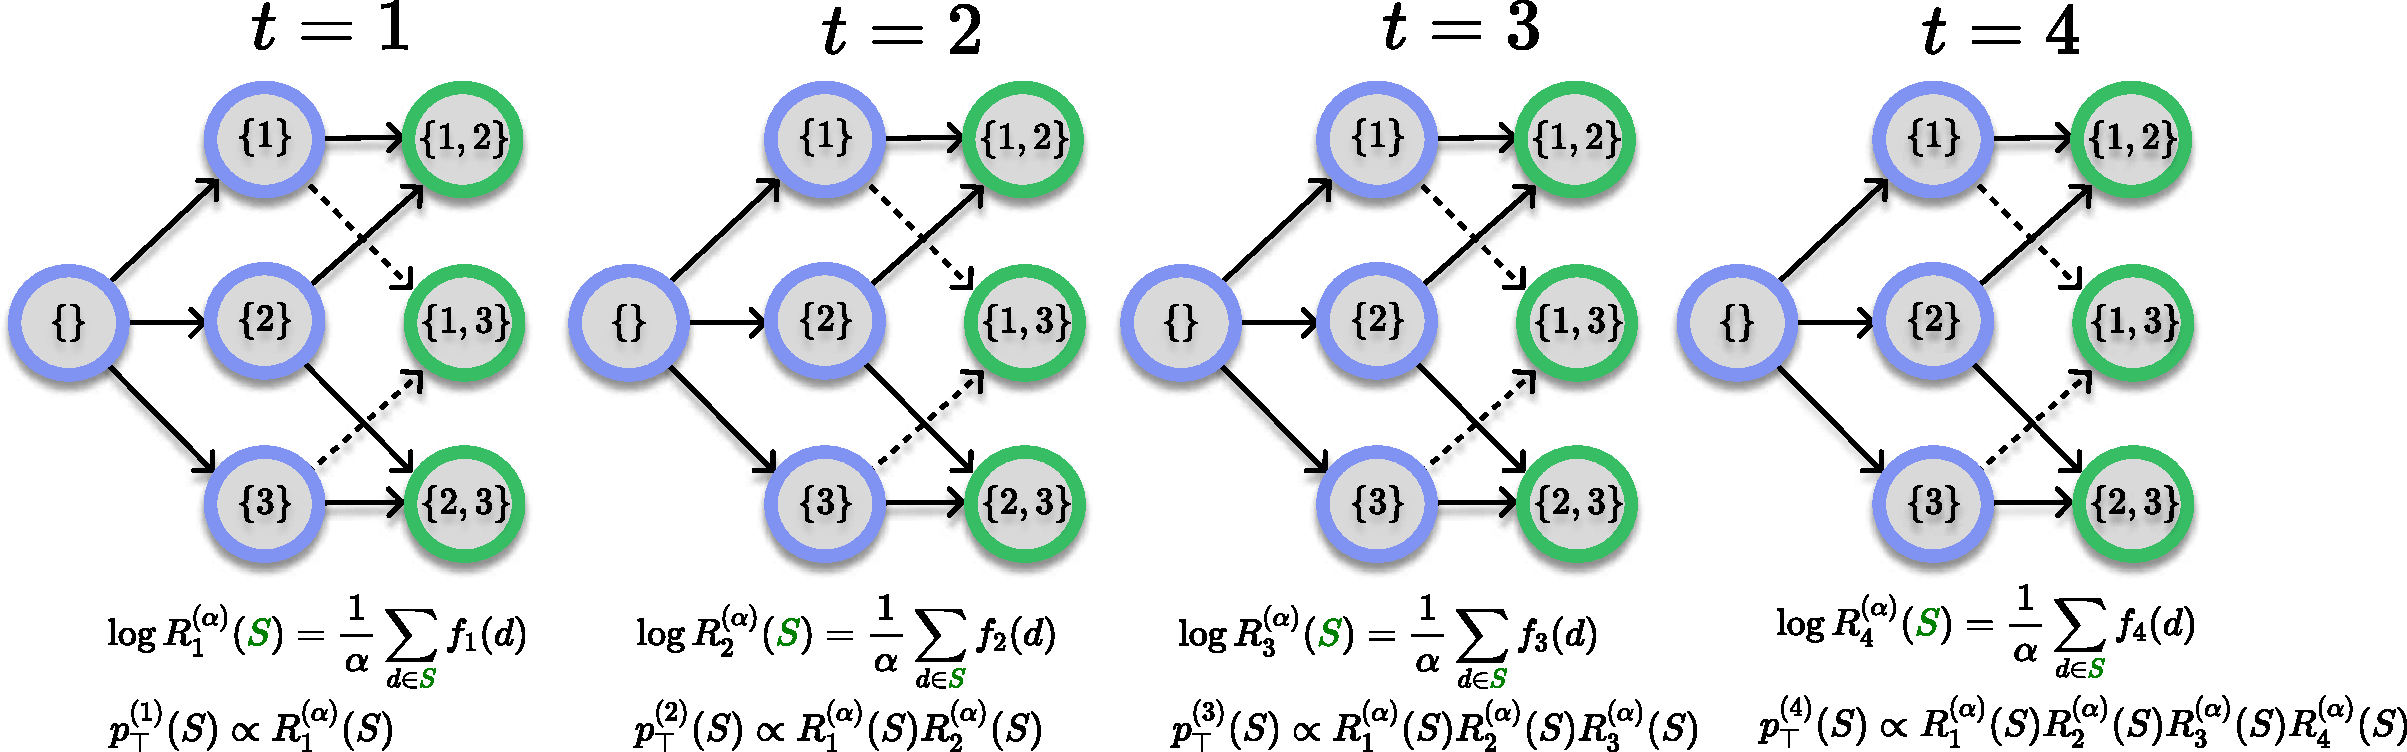
\includegraphics[width=.7\linewidth]{figures_rebuttal/diagram_compressed.pdf}
    \caption{\textbf{Illustration of the task of generating sets} of size $|S| = 2$ with elements in $\{1, 2, 3\}$. On each streaming update, a novel reward function $R_{i}^{(\alpha)}$ is observed; a small value of $\alpha$ entails a more sparse and harder-to-sample-from distribution. Terminal states \textcolor{teal}{$\mathcal{X}$} are illustrated in \textcolor{teal}{green} and non-terminal states are depicted in \textcolor{bleudefrance}{blue}. At the $t$th iteration, we learn a generative model $p_{\top}^{(t)}$ sampling $S \in \mathcal{X}$ proportionally to $\prod_{1 \le i \le t} R_{t}^{(\alpha)}(S)$. \looseness=-1}
    \label{fig:setgenerations}
\end{figure}

\pp{Experimental setup.} We fixed $d = 24$ and $S = 18$. To parameterize the forward policy, we implemented an two-layer neural network with a 128-dimensional latent embedding. For the streaming updates, we fixed $\alpha = 1$ and randomly sampled the objects' utilities at each novel iteration. We trained the model by minimizing the KL streaming criterion. 

\pp{GFlowNet's design.} To generate a set $x \in \mathcal{X}$, we iteratively add elements randomly sampled from $\mathcal{I}$ to an initially empty $x$ until $x$ has size $S$; see \autoref{fig:setgenerations}. The forward policy is parameterized as a two-layer neural network and the backward policy is fixed as an uniform distribution. 

\subsection{Linear preference learning with integer-valued features} 

\pp{Experimental setup.} We assume that $x \in [[0, 4]]^{d}$ and $d = 24$ and that the data was simulated from the observational model. At each streaming round, a novel and independent data set was simulated and the model was trained by minimizing the SB loss. To parameterize the forward policy, we implemented an MLP with 2 64-dimensional layers receiving the padded parameter $x$ as an input and returning a probability distribution over $[[0, 4]]$.    

\pp{GFlowNet's design.} The generative process implemented by the GFlowNet consists of, starting at an initially empty state $x_{o}$, iteratively sampling a value from $[[0, 10]]$ and appending this value to the current state until its length reaches $d$. To parameterize the forward policy, we use an MLP with two 64-dimensional layers that receives the padded state as a fixed-size input. 

\subsection{Online Bayesian phylogenetic inference} 

\pp{Experimental setup.} We assume the observational data follow the J\&C69 mutation model with an instantaneous mutation rate of $\lambda = 5 \cdot 10^{-3}$. The data was synthetically generated from the corresponding observational model conditioned on a randomly sampled tree with 7 leaves, and this process was repeated at each streaming round. To illustrate the computational gains enacted by the implementation of SB-GFlowNets in \autoref{tab:phy:t}, we considered updating a GFlowNet trained on an initially large data set according to the newly observed and relatively small biological sequences, which is a common challenge faced by practitioners. Then, by avoiding the additional log-likelihood evaluations, we achieved significantly faster inference.

\pp{GFlowNet's design.} A state consists of a forest of complete binary trees. Initially, all leaves are roots of their own singleton trees and, at each iteration of the generative process, we select two trees and join their roots to a newly added unlabelled node. This procedure is finished when all leaves are connected; see \cite[Figure 1]{zhou2024phylogfn} for an illustration of this generative process. To parameterize $p_{F}$, we use a graph isomorphism network (GIN; \cite{xu2018powerful}); the backward policy is fixed as uniform. 

\subsection{Bayesian structure learning} 

\pp{Experimental setup.} We sample each component of the error terms $\boldsymbol{\epsilon}$ from a zero-centered Gaussian distribution with standard deviation $\sigma = 5 \cdot 10^{-2}$. Also, we select a random Bayesian network from a directed configuration model \cite{newman} and draw the components $\beta$ from a corresponding standard Gaussian distribution to define the true data-generating process. 
To parameterize the policy network, we use an MLP with 2 128-dimensional layers receiving the DAG's flattened adjacency matrix as input. 
\looseness=-1  

\pp{GFlowNet's design.} We adopt \citet{deleu2022bayesian}'s DAG-GFlowNet. 
In a nutshell, the generative process starts at an edgeless graph and each transition either adds an edge to the current state or triggers a stop. 
To ensure the acyclicity of the generated samples, we follow \cite[Appendix C]{deleu2022bayesian} and iteratively update a binary vector $\mathbf{m} \in \{1, 0\}^{d \times d}$ indicating which edges in the adjacency matrix can be safely added to the current state without forming cycles. \looseness=-1 

\section{On the permutation invariance of SB-GFlowNets}


\begin{figure}[h!]
    \centering
    \begin{subfigure}{.4\textwidth} 
        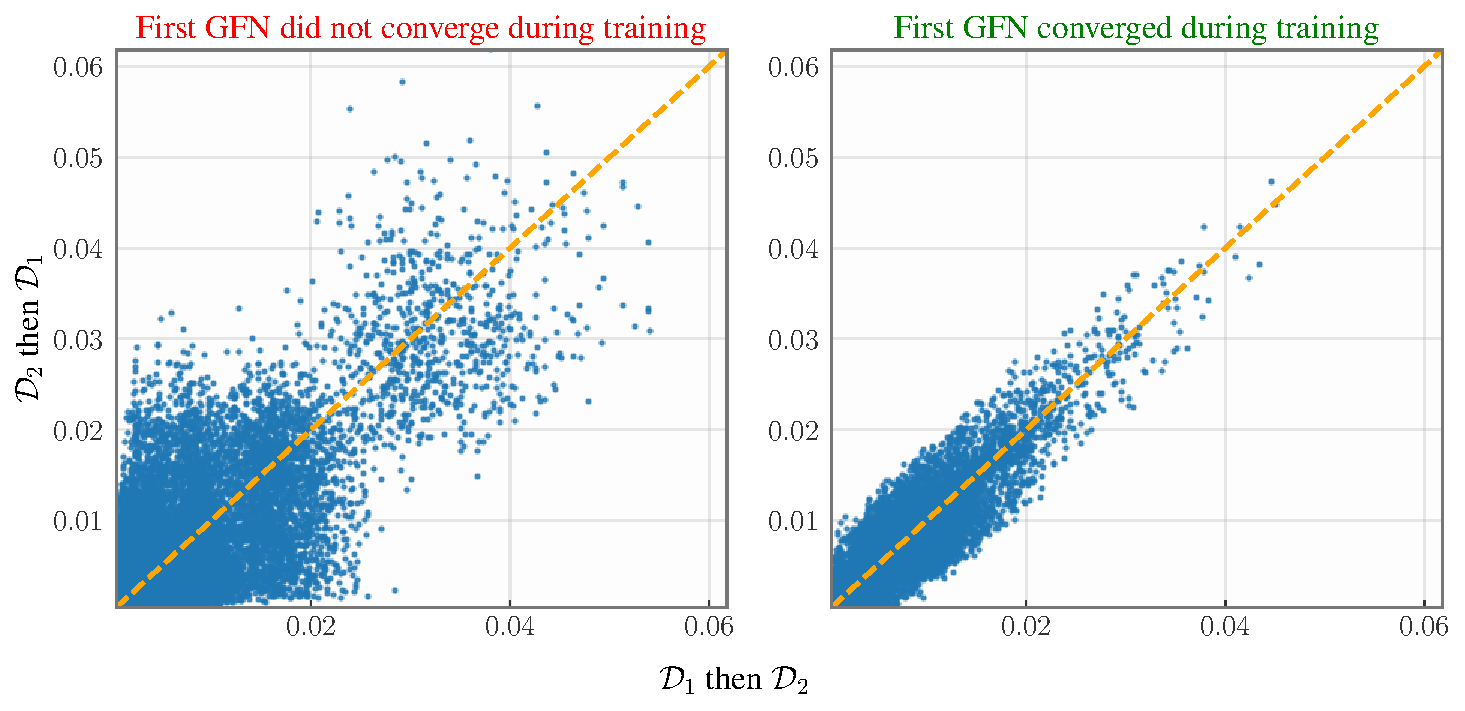
\includegraphics[width=\linewidth]{figures_rebuttal/streaming_eval_permutation.pdf}
        \caption{Phylogenetic inference.}
    \end{subfigure}
    \begin{subfigure}{.4\textwidth} 
        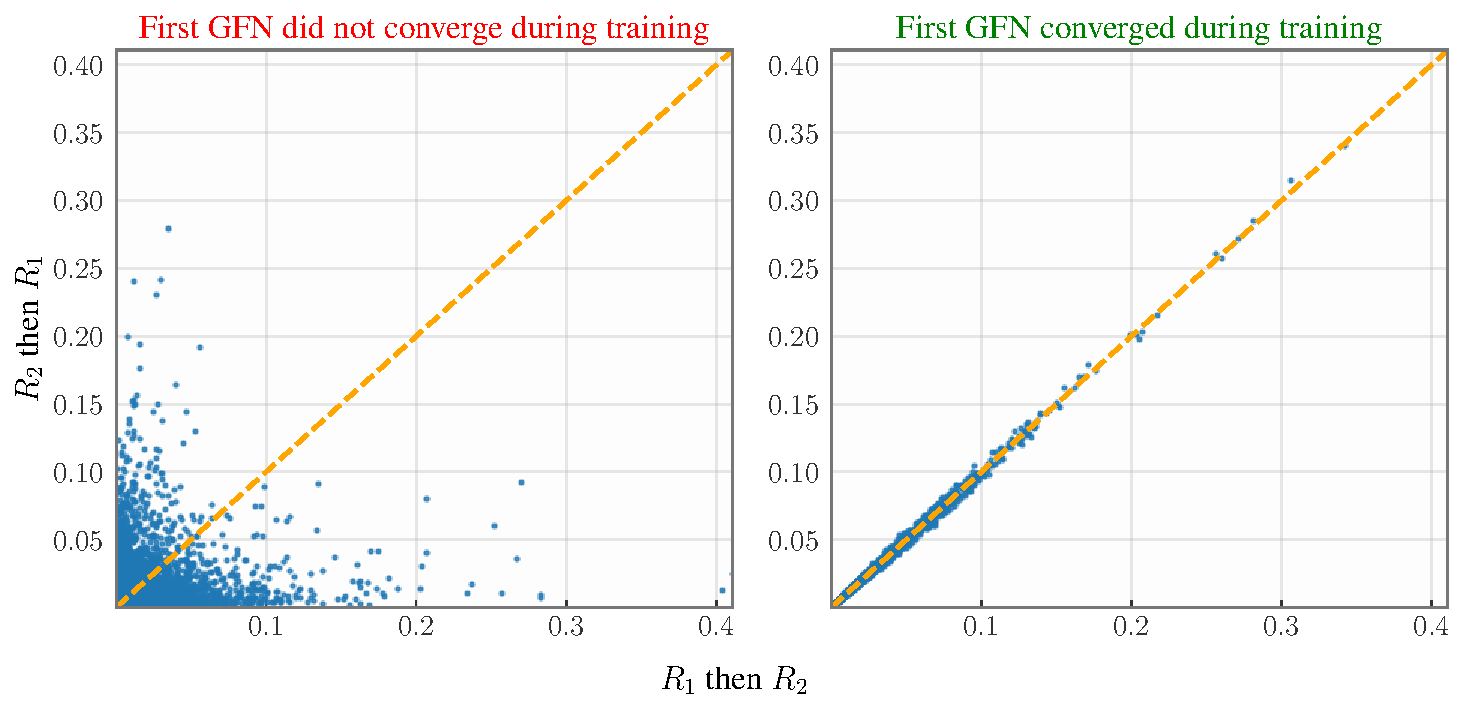
\includegraphics[width=\linewidth]{figures_rebuttal/streaming_eval_permutation_sets.pdf}
        \caption{Set generation.} 
    \end{subfigure}
    \caption{\textbf{Permutation invariance of SB-GFlowNets} for phylogenetics (a) and set generation (b). When the first GFlowNet is not adequately trained, the learned distribution after two streaming updates depends on the ordering of the observed datasets (\textcolor{red}{left} (a), \textcolor{red}{left} (b)). In contrast, when both the first and second GFlowNets are accurate, the resulting distribution is approximately invariant to the data permutation (\textcolor{teal}{right} (a), \textcolor{teal}{right} (b)). \looseness=-1}
    \label{fig:permutations}
\end{figure}

Exchangeability is a natural property of each case study we presented in the main text. 
We thus ask: are SB-GFlowNets permutation invariant? 
Clearly, the distribution learned by a SB-GFlowNet does not depend on the order in which the data sets are observed when the SB condition is satisfied at each streaming update; this is a direct consequence of \autoref{prop:streaming}. On the other hand, permutation invariance is not guaranteed when the learning objectives are only imperfectly minimized; see \autoref{fig:permutations} for an extreme example. 
To the best of our knowledge, however, this sensibility to data ordering is a property of every approximate streaming Bayesian inference method, e.g., \cite{Broderick13, Dinh2017}. 
\looseness=-1  
% In view of \autoref{prop:streaming}, it is clear  

\clearpage

\section*{NeurIPS Paper Checklist}

%%% END INSTRUCTIONS %%%


\begin{enumerate}

\item {\bf Claims}
    \item[] Question: Do the main claims made in the abstract and introduction accurately reflect the paper's contributions and scope?
    \item[] Answer: \answerYes{}
    \item[] Justification: Our claims are supported by proofs in \autoref{sec:app:proofs} and experiments in \autoref{sec:experiments}.
    \item[] Guidelines:
    \begin{itemize}
        \item The answer NA means that the abstract and introduction do not include the claims made in the paper.
        \item The abstract and/or introduction should clearly state the claims made, including the contributions made in the paper and important assumptions and limitations. A No or NA answer to this question will not be perceived well by the reviewers. 
        \item The claims made should match theoretical and experimental results, and reflect how much the results can be expected to generalize to other settings. 
        \item It is fine to include aspirational goals as motivation as long as it is clear that these goals are not attained by the paper. 
    \end{itemize}

\item {\bf Limitations}
    \item[] Question: Does the paper discuss the limitations of the work performed by the authors?
    \item[] Answer: \answerYes{} % Replace by \answerYes{}, \answerNo{}, or \answerNA{}.
    \item[] Justification: The middle paragraph in \autoref{sec:aaa} discusses limitations.
    \item[] Guidelines:
    \begin{itemize}
        \item The answer NA means that the paper has no limitation while the answer No means that the paper has limitations, but those are not discussed in the paper. 
        \item The authors are encouraged to create a separate "Limitations" section in their paper.
        \item The paper should point out any strong assumptions and how robust the results are to violations of these assumptions (e.g., independence assumptions, noiseless settings, model well-specification, asymptotic approximations only holding locally). The authors should reflect on how these assumptions might be violated in practice and what the implications would be.
        \item The authors should reflect on the scope of the claims made, e.g., if the approach was only tested on a few datasets or with a few runs. In general, empirical results often depend on implicit assumptions, which should be articulated.
        \item The authors should reflect on the factors that influence the performance of the approach. For example, a facial recognition algorithm may perform poorly when image resolution is low or images are taken in low lighting. Or a speech-to-text system might not be used reliably to provide closed captions for online lectures because it fails to handle technical jargon.
        \item The authors should discuss the computational efficiency of the proposed algorithms and how they scale with dataset size.
        \item If applicable, the authors should discuss possible limitations of their approach to address problems of privacy and fairness.
        \item While the authors might fear that complete honesty about limitations might be used by reviewers as grounds for rejection, a worse outcome might be that reviewers discover limitations that aren't acknowledged in the paper. The authors should use their best judgment and recognize that individual actions in favor of transparency play an important role in developing norms that preserve the integrity of the community. Reviewers will be specifically instructed to not penalize honesty concerning limitations.
    \end{itemize}

\item {\bf Theory Assumptions and Proofs}
    \item[] Question: For each theoretical result, does the paper provide the full set of assumptions and a complete (and correct) proof?
    \item[] Answer: \answerYes{} % Replace by \answerYes{}, \answerNo{}, or \answerNA{}.
    \item[] Justification: Assumptions are clearly stated in the statements, and \autoref{sec:app:proofs}.
    \item[] Guidelines:
    \begin{itemize}
        \item The answer NA means that the paper does not include theoretical results. 
        \item All the theorems, formulas, and proofs in the paper should be numbered and cross-referenced.
        \item All assumptions should be clearly stated or referenced in the statement of any theorems.
        \item The proofs can either appear in the main paper or the supplemental material, but if they appear in the supplemental material, the authors are encouraged to provide a short proof sketch to provide intuition. 
        \item Inversely, any informal proof provided in the core of the paper should be complemented by formal proofs provided in appendix or supplemental material.
        \item Theorems and Lemmas that the proof relies upon should be properly referenced. 
    \end{itemize}

    \item {\bf Experimental Result Reproducibility}
    \item[] Question: Does the paper fully disclose all the information needed to reproduce the main experimental results of the paper to the extent that it affects the main claims and/or conclusions of the paper (regardless of whether the code and data are provided or not)?
    \item[] Answer: \answerYes{} % Replace by \answerYes{}, \answerNo{}, or \answerNA{}.
    \item[] Justification: Details are provided in \autoref{sec:app:experiments}.
    \item[] Guidelines:
    \begin{itemize}
        \item The answer NA means that the paper does not include experiments.
        \item If the paper includes experiments, a No answer to this question will not be perceived well by the reviewers: Making the paper reproducible is important, regardless of whether the code and data are provided or not.
        \item If the contribution is a dataset and/or model, the authors should describe the steps taken to make their results reproducible or verifiable. 
        \item Depending on the contribution, reproducibility can be accomplished in various ways. For example, if the contribution is a novel architecture, describing the architecture fully might suffice, or if the contribution is a specific model and empirical evaluation, it may be necessary to either make it possible for others to replicate the model with the same dataset, or provide access to the model. In general. releasing code and data is often one good way to accomplish this, but reproducibility can also be provided via detailed instructions for how to replicate the results, access to a hosted model (e.g., in the case of a large language model), releasing of a model checkpoint, or other means that are appropriate to the research performed.
        \item While NeurIPS does not require releasing code, the conference does require all submissions to provide some reasonable avenue for reproducibility, which may depend on the nature of the contribution. For example
        \begin{enumerate}
            \item If the contribution is primarily a new algorithm, the paper should make it clear how to reproduce that algorithm.
            \item If the contribution is primarily a new model architecture, the paper should describe the architecture clearly and fully.
            \item If the contribution is a new model (e.g., a large language model), then there should either be a way to access this model for reproducing the results or a way to reproduce the model (e.g., with an open-source dataset or instructions for how to construct the dataset).
            \item We recognize that reproducibility may be tricky in some cases, in which case authors are welcome to describe the particular way they provide for reproducibility. In the case of closed-source models, it may be that access to the model is limited in some way (e.g., to registered users), but it should be possible for other researchers to have some path to reproducing or verifying the results.
        \end{enumerate}
    \end{itemize}


\item {\bf Open access to data and code}
    \item[] Question: Does the paper provide open access to the data and code, with sufficient instructions to faithfully reproduce the main experimental results, as described in supplemental material?
    \item[] Answer: \answerYes{} % Replace by \answerYes{}, \answerNo{}, or \answerNA{}.
    \item[] Justification: Provided in a zip file.  
    \item[] Guidelines:
    \begin{itemize}
        \item The answer NA means that paper does not include experiments requiring code.
        \item Please see the NeurIPS code and data submission guidelines (\url{https://nips.cc/public/guides/CodeSubmissionPolicy}) for more details.
        \item While we encourage the release of code and data, we understand that this might not be possible, so “No” is an acceptable answer. Papers cannot be rejected simply for not including code, unless this is central to the contribution (e.g., for a new open-source benchmark).
        \item The instructions should contain the exact command and environment needed to run to reproduce the results. See the NeurIPS code and data submission guidelines (\url{https://nips.cc/public/guides/CodeSubmissionPolicy}) for more details.
        \item The authors should provide instructions on data access and preparation, including how to access the raw data, preprocessed data, intermediate data, and generated data, etc.
        \item The authors should provide scripts to reproduce all experimental results for the new proposed method and baselines. If only a subset of experiments are reproducible, they should state which ones are omitted from the script and why.
        \item At submission time, to preserve anonymity, the authors should release anonymized versions (if applicable).
        \item Providing as much information as possible in supplemental material (appended to the paper) is recommended, but including URLs to data and code is permitted.
    \end{itemize}


\item {\bf Experimental Setting/Details}
    \item[] Question: Does the paper specify all the training and test details (e.g., data splits, hyperparameters, how they were chosen, type of optimizer, etc.) necessary to understand the results?
    \item[] Answer: \answerYes{} % Replace by \answerYes{}, \answerNo{}, or \answerNA{}.
    \item[] Justification: Provided in \autoref{sec:app:experiments}.
    \item[] Guidelines:
    \begin{itemize}
        \item The answer NA means that the paper does not include experiments.
        \item The experimental setting should be presented in the core of the paper to a level of detail that is necessary to appreciate the results and make sense of them.
        \item The full details can be provided either with the code, in appendix, or as supplemental material.
    \end{itemize}

\item {\bf Experiment Statistical Significance}
    \item[] Question: Does the paper report error bars suitably and correctly defined or other appropriate information about the statistical significance of the experiments?
    \item[] Answer: \answerYes{} % Replace by \answerYes{}, \answerNo{}, or \answerNA{}.
    \item[] Justification: In general, plots count on error bars and tables count on standard deviation.
    \item[] Guidelines:
    \begin{itemize}
        \item The answer NA means that the paper does not include experiments.
        \item The authors should answer "Yes" if the results are accompanied by error bars, confidence intervals, or statistical significance tests, at least for the experiments that support the main claims of the paper.
        \item The factors of variability that the error bars are capturing should be clearly stated (for example, train/test split, initialization, random drawing of some parameter, or overall run with given experimental conditions).
        \item The method for calculating the error bars should be explained (closed form formula, call to a library function, bootstrap, etc.)
        \item The assumptions made should be given (e.g., Normally distributed errors).
        \item It should be clear whether the error bar is the standard deviation or the standard error of the mean.
        \item It is OK to report 1-sigma error bars, but one should state it. The authors should preferably report a 2-sigma error bar than state that they have a 96\% CI, if the hypothesis of Normality of errors is not verified.
        \item For asymmetric distributions, the authors should be careful not to show in tables or figures symmetric error bars that would yield results that are out of range (e.g. negative error rates).
        \item If error bars are reported in tables or plots, The authors should explain in the text how they were calculated and reference the corresponding figures or tables in the text.
    \end{itemize}

\item {\bf Experiments Compute Resources}
    \item[] Question: For each experiment, does the paper provide sufficient information on the computer resources (type of compute workers, memory, time of execution) needed to reproduce the experiments?
    \item[] Answer: \answerYes{} % Replace by \answerYes{}, \answerNo{}, or \answerNA{}.
    \item[] Justification: First paragraph of \autoref{sec:app:experiments}.
    \item[] Guidelines:
    \begin{itemize}
        \item The answer NA means that the paper does not include experiments.
        \item The paper should indicate the type of compute workers CPU or GPU, internal cluster, or cloud provider, including relevant memory and storage.
        \item The paper should provide the amount of compute required for each of the individual experimental runs as well as estimate the total compute. 
        \item The paper should disclose whether the full research project required more compute than the experiments reported in the paper (e.g., preliminary or failed experiments that didn't make it into the paper). 
    \end{itemize}
    
\item {\bf Code Of Ethics}
    \item[] Question: Does the research conducted in the paper conform, in every respect, with the NeurIPS Code of Ethics \url{https://neurips.cc/public/EthicsGuidelines}?
    \item[] Answer: \answerYes{} % Replace by \answerYes{}, \answerNo{}, or \answerNA{}.
    \item[] Justification: Our submission follows the NeurIPS ethical guidelines.
    \item[] Guidelines:
    \begin{itemize}
        \item The answer NA means that the authors have not reviewed the NeurIPS Code of Ethics.
        \item If the authors answer No, they should explain the special circumstances that require a deviation from the Code of Ethics.
        \item The authors should make sure to preserve anonymity (e.g., if there is a special consideration due to laws or regulations in their jurisdiction).
    \end{itemize}


\item {\bf Broader Impacts}
    \item[] Question: Does the paper discuss both potential positive societal impacts and negative societal impacts of the work performed?
    \item[] Answer: \answerYes{} % Replace by \answerYes{}, \answerNo{}, or \answerNA{}.
    \item[] Justification: We provide a perspective on broader impacts in \autoref{sec:aaa}, but do not foresee any direct negative societal impact.
    \item[] Guidelines:
    \begin{itemize}
        \item The answer NA means that there is no societal impact of the work performed.
        \item If the authors answer NA or No, they should explain why their work has no societal impact or why the paper does not address societal impact.
        \item Examples of negative societal impacts include potential malicious or unintended uses (e.g., disinformation, generating fake profiles, surveillance), fairness considerations (e.g., deployment of technologies that could make decisions that unfairly impact specific groups), privacy considerations, and security considerations.
        \item The conference expects that many papers will be foundational research and not tied to particular applications, let alone deployments. However, if there is a direct path to any negative applications, the authors should point it out. For example, it is legitimate to point out that an improvement in the quality of generative models could be used to generate deepfakes for disinformation. On the other hand, it is not needed to point out that a generic algorithm for optimizing neural networks could enable people to train models that generate Deepfakes faster.
        \item The authors should consider possible harms that could arise when the technology is being used as intended and functioning correctly, harms that could arise when the technology is being used as intended but gives incorrect results, and harms following from (intentional or unintentional) misuse of the technology.
        \item If there are negative societal impacts, the authors could also discuss possible mitigation strategies (e.g., gated release of models, providing defenses in addition to attacks, mechanisms for monitoring misuse, mechanisms to monitor how a system learns from feedback over time, improving the efficiency and accessibility of ML).
    \end{itemize}
    
\item {\bf Safeguards}
    \item[] Question: Does the paper describe safeguards that have been put in place for responsible release of data or models that have a high risk for misuse (e.g., pretrained language models, image generators, or scraped datasets)?
    \item[] Answer: \answerNA{} % Replace by \answerYes{}, \answerNo{}, or \answerNA{}.
    \item[] Justification: We do not foresee any direct risk stemming from our work.
    \item[] Guidelines:
    \begin{itemize}
        \item The answer NA means that the paper poses no such risks.
        \item Released models that have a high risk for misuse or dual-use should be released with necessary safeguards to allow for controlled use of the model, for example by requiring that users adhere to usage guidelines or restrictions to access the model or implementing safety filters. 
        \item Datasets that have been scraped from the Internet could pose safety risks. The authors should describe how they avoided releasing unsafe images.
        \item We recognize that providing effective safeguards is challenging, and many papers do not require this, but we encourage authors to take this into account and make a best faith effort.
    \end{itemize}

\item {\bf Licenses for existing assets}
    \item[] Question: Are the creators or original owners of assets (e.g., code, data, models), used in the paper, properly credited and are the license and terms of use explicitly mentioned and properly respected?
    \item[] Answer: \answerNA{} % Replace by \answerYes{}, \answerNo{}, or \answerNA{}.
    \item[] Justification: All code was made by the authors
    \item[] Guidelines:
    \begin{itemize}
        \item The answer NA means that the paper does not use existing assets.
        \item The authors should cite the original paper that produced the code package or dataset.
        \item The authors should state which version of the asset is used and, if possible, include a URL.
        \item The name of the license (e.g., CC-BY 4.0) should be included for each asset.
        \item For scraped data from a particular source (e.g., website), the copyright and terms of service of that source should be provided.
        \item If assets are released, the license, copyright information, and terms of use in the package should be provided. For popular datasets, \url{paperswithcode.com/datasets} has curated licenses for some datasets. Their licensing guide can help determine the license of a dataset.
        \item For existing datasets that are re-packaged, both the original license and the license of the derived asset (if it has changed) should be provided.
        \item If this information is not available online, the authors are encouraged to reach out to the asset's creators.
    \end{itemize}

\item {\bf New Assets}
    \item[] Question: Are new assets introduced in the paper well documented and is the documentation provided alongside the assets?
    \item[] Answer: \answerNA{} % Replace by \answerYes{}, \answerNo{}, or \answerNA{}.
    \item[] Justification: No new assets.
    \item[] Guidelines:
    \begin{itemize}
        \item The answer NA means that the paper does not release new assets.
        \item Researchers should communicate the details of the dataset/code/model as part of their submissions via structured templates. This includes details about training, license, limitations, etc. 
        \item The paper should discuss whether and how consent was obtained from people whose asset is used.
        \item At submission time, remember to anonymize your assets (if applicable). You can either create an anonymized URL or include an anonymized zip file.
    \end{itemize}

\item {\bf Crowdsourcing and Research with Human Subjects}
    \item[] Question: For crowdsourcing experiments and research with human subjects, does the paper include the full text of instructions given to participants and screenshots, if applicable, as well as details about compensation (if any)? 
    \item[] Answer: \answerNA{} % Replace by \answerYes{}, \answerNo{}, or \answerNA{}.
    \item[] Justification: No experiments with human subjects.
    \item[] Guidelines:
    \begin{itemize}
        \item The answer NA means that the paper does not involve crowdsourcing nor research with human subjects.
        \item Including this information in the supplemental material is fine, but if the main contribution of the paper involves human subjects, then as much detail as possible should be included in the main paper. 
        \item According to the NeurIPS Code of Ethics, workers involved in data collection, curation, or other labor should be paid at least the minimum wage in the country of the data collector. 
    \end{itemize}

\item {\bf Institutional Review Board (IRB) Approvals or Equivalent for Research with Human Subjects}
    \item[] Question: Does the paper describe potential risks incurred by study participants, whether such risks were disclosed to the subjects, and whether Institutional Review Board (IRB) approvals (or an equivalent approval/review based on the requirements of your country or institution) were obtained?
    \item[] Answer: \answerNA{} % Replace by \answerYes{}, \answerNo{}, or \answerNA{}.
    \item[] Justification: No experiments with human subjects.
    \item[] Guidelines:
    \begin{itemize}
        \item The answer NA means that the paper does not involve crowdsourcing nor research with human subjects.
        \item Depending on the country in which research is conducted, IRB approval (or equivalent) may be required for any human subjects research. If you obtained IRB approval, you should clearly state this in the paper. 
        \item We recognize that the procedures for this may vary significantly between institutions and locations, and we expect authors to adhere to the NeurIPS Code of Ethics and the guidelines for their institution. 
        \item For initial submissions, do not include any information that would break anonymity (if applicable), such as the institution conducting the review.
    \end{itemize}

\end{enumerate}


\end{document}